\chapter{HASIL DAN PEMBAHASAN}
\label{chap:hasilpembahasan}

% Ubah bagian-bagian berikut dengan isi dari hasil dan pembahasan

Pada bab ini dipaparkan hasil dan analisa dari pelaksanaan tiap tahapan pada metodologi, serta dipaparkan mengenai skenario pengujian dan evaluasi pengujiannya. Pengujian dilakukan guna mengetahui tingkat kesalahan dan menarik kesimpulan dari metodologi serta analisis yang telah dibuat. Tahapan skenario pengujian meliputi hal berikut, yaitu: \par

\begin{enumerate}[nolistsep]
  \item Pengujian menggunakan \textit{pretrained weight} model yang bervariasi.
  \item Pengujian menggunakan \textit{input} citra tulisan dari responden berbeda.
  \item Pengujian menggunakan \textit{input} citra dengan jarak pengambilan citra bervariasi.
  \item Pengujian menggunakan \textit{input} citra dengan pencahayaan pengambilan citra bervariasi.
\end{enumerate}

Dengan hasil metodologi serta pelaksanaan skenario-skenario pengujian yang akan dipaparkan pada bab 4 ini, diharapkan mendapatkan hasil dan analisa sehingga dapat ditarik kesimpulan dari pelaksanaan tugas akhir ini. \par

\section{Hasil Metodologi}
\label{sec:hasilmetodologi}

Pada metodologi terdapat blok-blok diagram dan telah dilakukan pelaksanaan tugas akhir sesuai dengan blok diagram tersebut. Adapun hasil dari tiap tahapan yang dilakukan pada blok diagram tersebut secara rinci akan dijelaskan pada sub berikut. \par
% ini dijelaskan sesuai dengan metodologi yang telah dibuat sebelumnya. \par

\subsection{Hasil Akuisisi Dataset}
\label{subsec:Hasilakuisisidataset}

Pada tahapan akuisisi dataset, secara umum pelaksanaannya terbagi dalam 3 tahapan yaitu pengumpulan citra tulisan tangan pada papan tulis, proses pelabelan, dan proses \textit{image pre-processing.} Pada tahapan akuisisi dataset, secara umum didapatkan hasil jumlah dataset seperti pada Tabel \ref*{tb:hasilakuisisidata} serta proses \textit{pre-process} secara singkat seperti pada Tabel \ref*{tb:checklistpreprocess}.

% //FIXME: perbarui detail preproses dataset
\begin{center}
  \begin{longtable}[c]{|l|l|}
    \hline
    \multicolumn{1}{|c|}{\textbf{Jenis \textit{Pre-Process}}} & \multicolumn{1}{c|}{\textbf{Keterangan}} \\ \hline
    \endfirsthead
    \endhead
    \textit{Auto Orient}                             & Diterapkan                                               \\ \hline
    \textit{Resize}                                  & \textit{Stretch to} 416x416                              \\ \hline
    \textit{Grayscale}                               & Diterapkan                                               \\ \hline
    \textit{Contrast}                                & \textit{Contrast Stretching}                             \\ \hline
    \textit{Filter Null}                             & Diterapkan                                               \\ \hline
    \textit{Blur}                                    & \textit{Random up to 8px}                                \\ \hline
    \textit{Noise}                                   & \textit{Random up to 2\% pixels}                         \\ \hline
    \textit{Bounding Box Rotation}                   & \textit{Random between -5\textdegree and +5\textdegree}  \\ \hline
    \caption{Tahapan Pre-Process yang Dilakukan}
    \label{tb:checklistpreprocess}\\
  \end{longtable}
\end{center}

% //FIXME: perbarui detail kelas dataset
\begin{center}
  \begin{longtable}[c]{|c|c|c|c|c|}
    \hline
    \textbf{Kelas} & \textbf{Jumlah Citra} & \multicolumn{1}{l|}{\textbf{Jumlah Anotasi}} & \multicolumn{1}{l|}{\textit{\textbf{Train Set}}} & \multicolumn{1}{l|}{\textit{\textbf{Validation Set}}} \\ \hline
    \endfirsthead
    \endhead
    *              & 36           & 540         & 29         & 7         \\ \hline
    =              & 50           & 750         & 45         & 5         \\ \hline
    0              & 50           & 750         & 45         & 5         \\ \hline
    1              & 50           & 750         & 45         & 5         \\ \hline
    2              & 50           & 750         & 45         & 5         \\ \hline
    3              & 50           & 750         & 45         & 5         \\ \hline
    4              & 50           & 750         & 45         & 5         \\ \hline
    5              & 50           & 750         & 45         & 5         \\ \hline
    6              & 50           & 750         & 45         & 5         \\ \hline
    7              & 50           & 750         & 45         & 5         \\ \hline
    8              & 50           & 750         & 45         & 5         \\ \hline
    9              & 50           & 750         & 45         & 5         \\ \hline
    A              & 50           & 750         & 45         & 5         \\ \hline
    B              & 50           & 750         & 45         & 5         \\ \hline
    D              & 50           & 750         & 45         & 5         \\ \hline
    E              & 50           & 750         & 45         & 5         \\ \hline
    G              & 50           & 750         & 45         & 5         \\ \hline
    I              & 50           & 750         & 45         & 5         \\ \hline
    J              & 50           & 750         & 45         & 5         \\ \hline
    K              & 50           & 750         & 45         & 5         \\ \hline
    L              & 50           & 750         & 45         & 5         \\ \hline
    M              & 50           & 750         & 45         & 5         \\ \hline
    N              & 50           & 750         & 45         & 5         \\ \hline
    P              & 50           & 750         & 45         & 5         \\ \hline
    R              & 50           & 750         & 45         & 5         \\ \hline
    S              & 50           & 750         & 45         & 5         \\ \hline
    T              & 50           & 750         & 45         & 5         \\ \hline
    U              & 50           & 750         & 45         & 5         \\ \hline
    V              & 50           & 750         & 45         & 5         \\ \hline
    \caption{Hasil Akuisisi Data}
    \label{tb:hasilakuisisidata}\\
  \end{longtable}
\end{center}

Secara spesifik, hasil dari tiap proses yang ada pada tahapan akuisisi dataset akan dijelaskan pada poin-poin berikut. \par

\subsubsection{Hasil Pengumpulan Citra Tulisan Tangan pada Papan Tulis}
\label{subsubsec:hasilpengumpulancitra}

Proses pengumpulan citra tulisan tangan papan tulis dilakukan dengan menuliskan sejumlah huruf, angka, dan simbol pada media papan tulis kemudian dilakukan proses pengambilan citra. Proses tersebut dilakukan secara berulang sampai jumlah tertentu untuk suatu kelas yang sama dan diulang kembali dengan kelas berbeda sampai seluruh jumlah kelas terpenuhi. Seluruh tulisan tangan pada papan tulis ditulis oleh 1 orang yang sama. Pada saat proses pengambilan citra, citra diambil dengan perangkat \textit{smartphone} yang detail spesifikasinya dapat dilihat pada Tabel \ref*{tb:spesifikasismartphone}. Dalam proses pengambilan citra, terdapat beberapa teknik berbeda dalam pengambilan citra, yaitu: pengambilan citra dengan intensitas cahaya berbeda (diatur menggunakan kamera penulis) dan pengambilan citra dengan sudut pengambilan citra yang berbeda. Hal tersebut dilakukan agar tiap kelas yang ada memiliki variasi sehingga ketika model diterapkan secara langsung dapat mendeteksi dari berbagai kondisi. Contoh hasil dari pengambilan citra dengan variasi intensitas cahaya dapat dilihat pada Gambar \ref{fig:intensitascitrabervariasi} dan contoh hasil dari pengambilan citra dengan variasi sudut pengambilan gambar dapat dilihat pada Gambar \ref*{fig:pengambilancitrabervariasi}.  \par

\begin{figure}[H]
  \begin{subfigure}{.5\textwidth}
    \centering
    \captionsetup{width=.8\linewidth}
    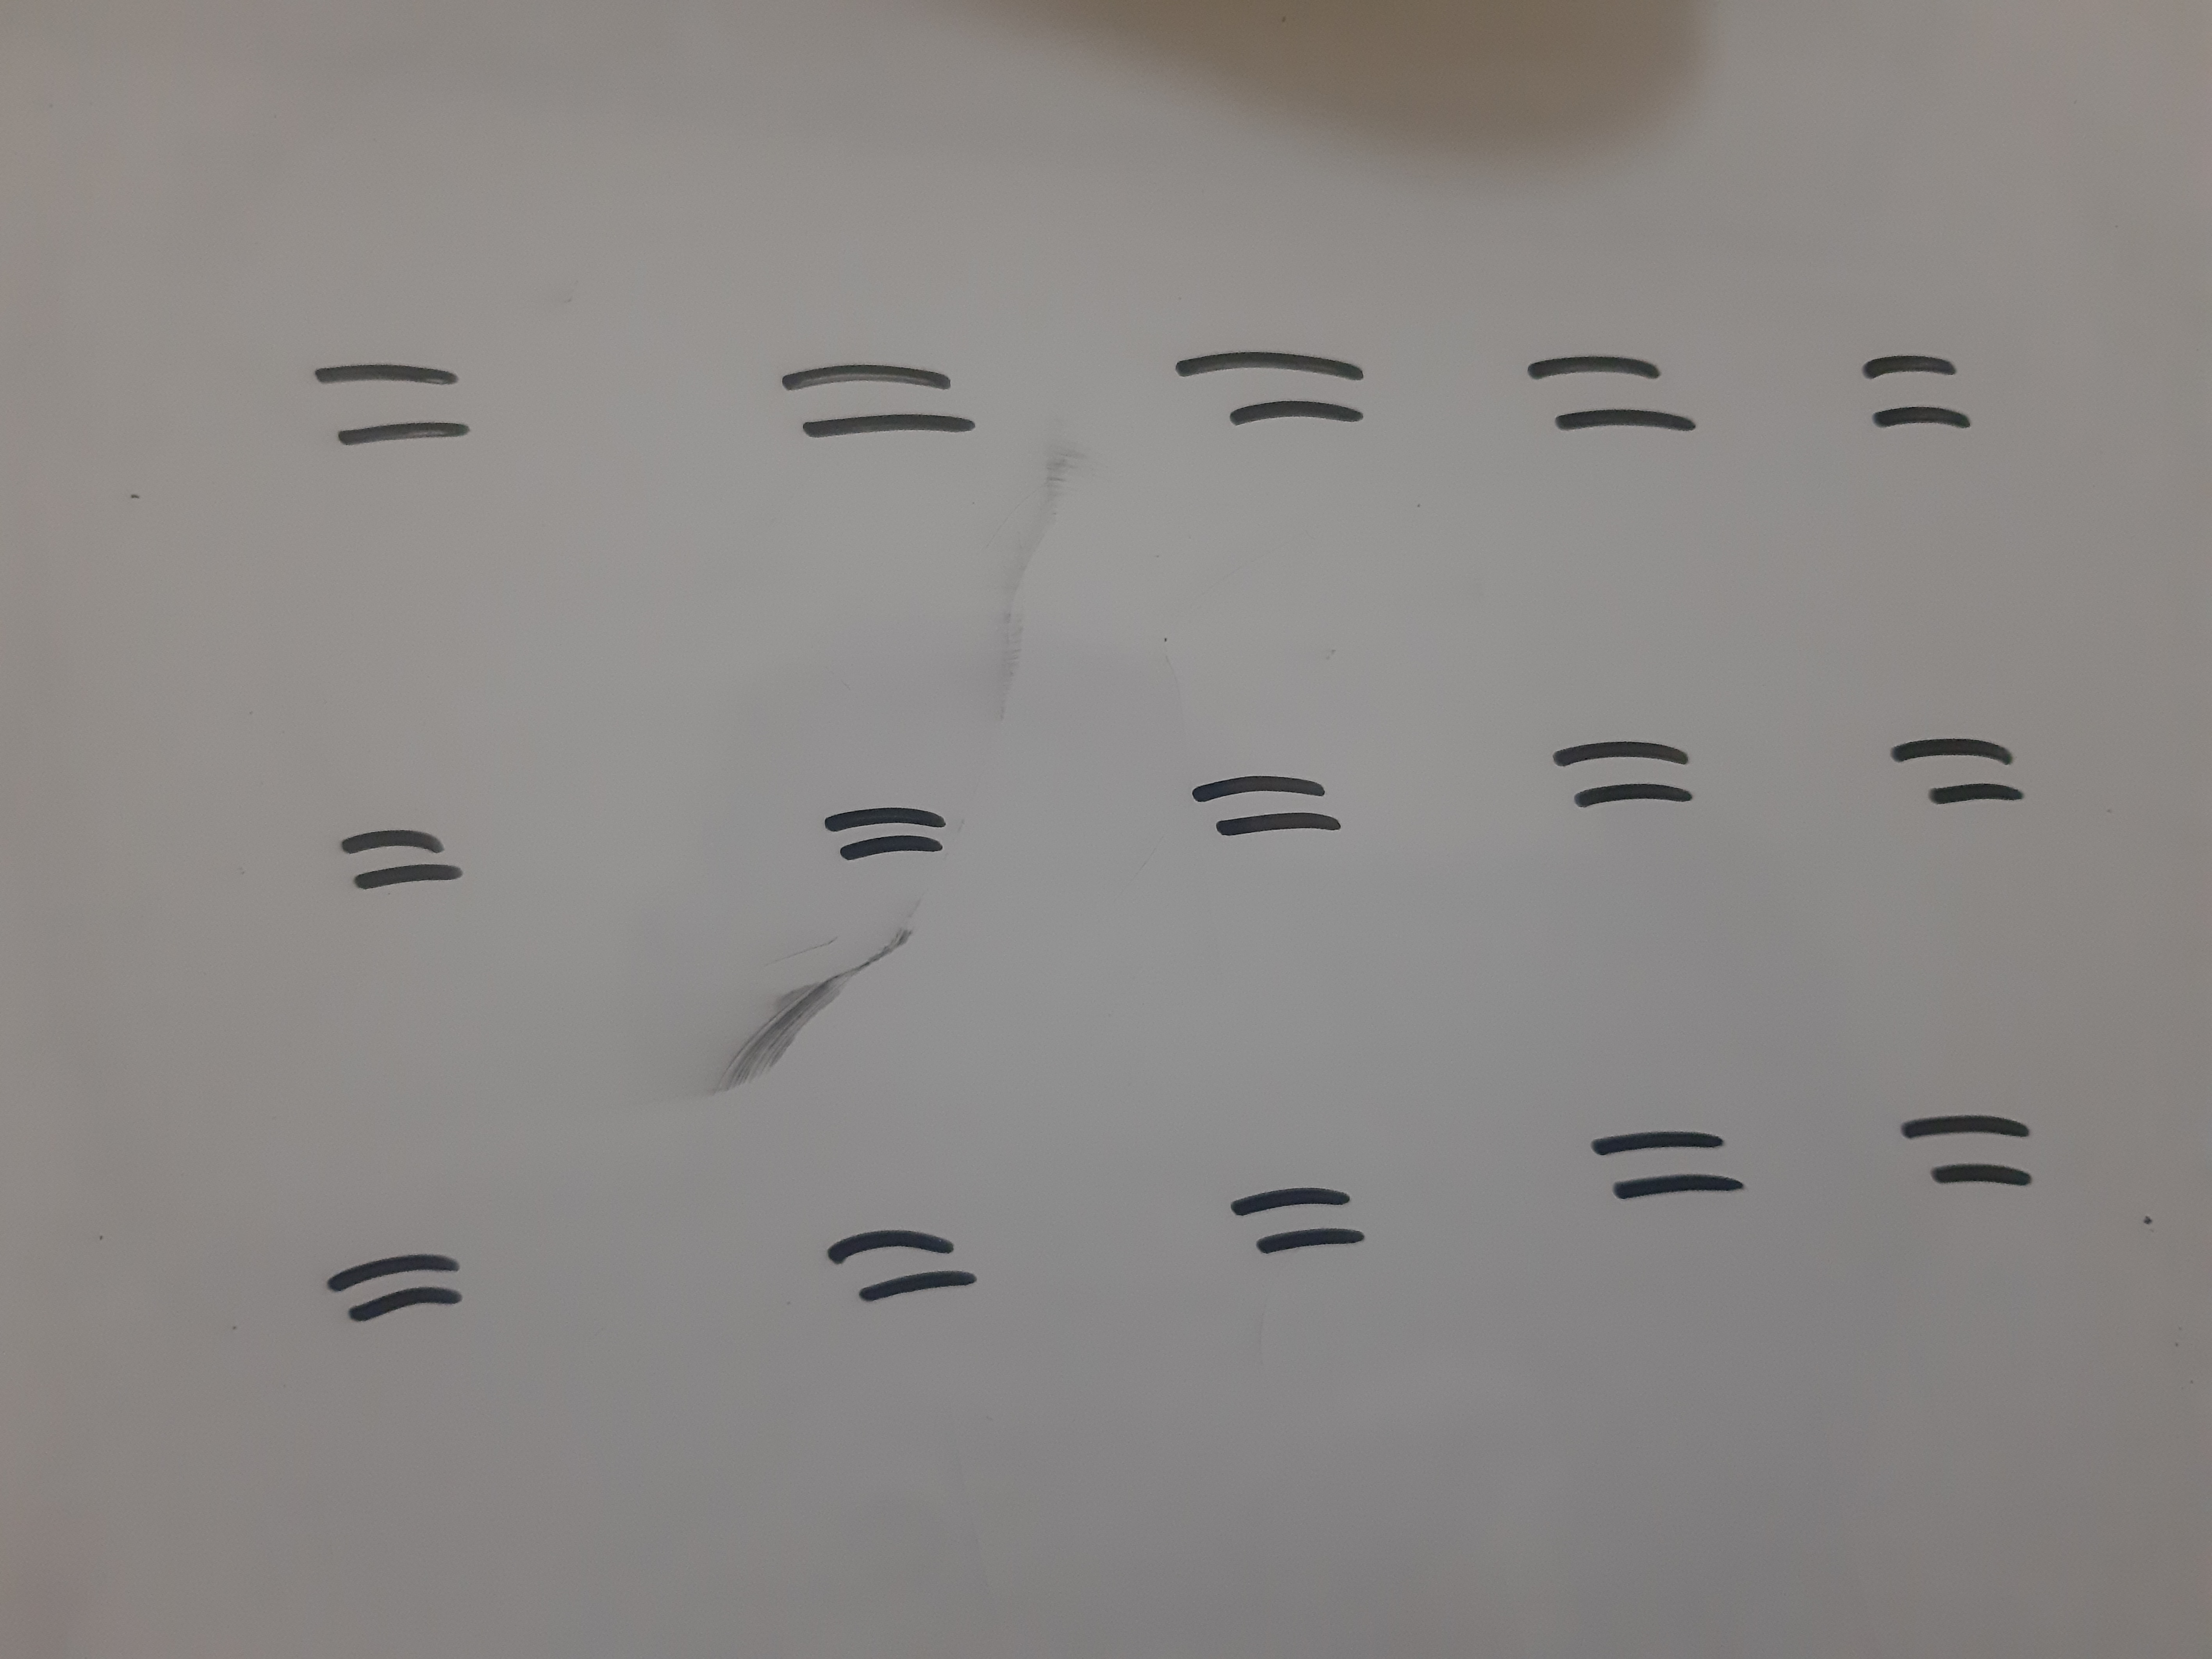
\includegraphics[width=.85\linewidth]{gambar/pengambilan_citra_terang.jpg}
    \caption{Pengambilan Citra dengan Kondisi Normal}
    \label{fig:citraterang}
  \end{subfigure}%
  \begin{subfigure}{.5\textwidth}
    \centering
    \captionsetup{width=.8\linewidth}
    \includegraphics[width=.85\linewidth]{gambar/pengambilan_citra_gelap.jpg}
    \caption{Pengambilan Citra dengan Kondisi \textit{Apperture} Kisaran -1 \textit{Steps.}}
    \label{fig:citragelap}
  \end{subfigure}
  \caption{Pengambilan Citra dengan Variasi Intensitas Cahaya}
  \label{fig:intensitascitrabervariasi}
\end{figure}

\begin{figure}[H]
  \begin{subfigure}{.5\textwidth}
    \centering
    \captionsetup{width=.8\linewidth}
    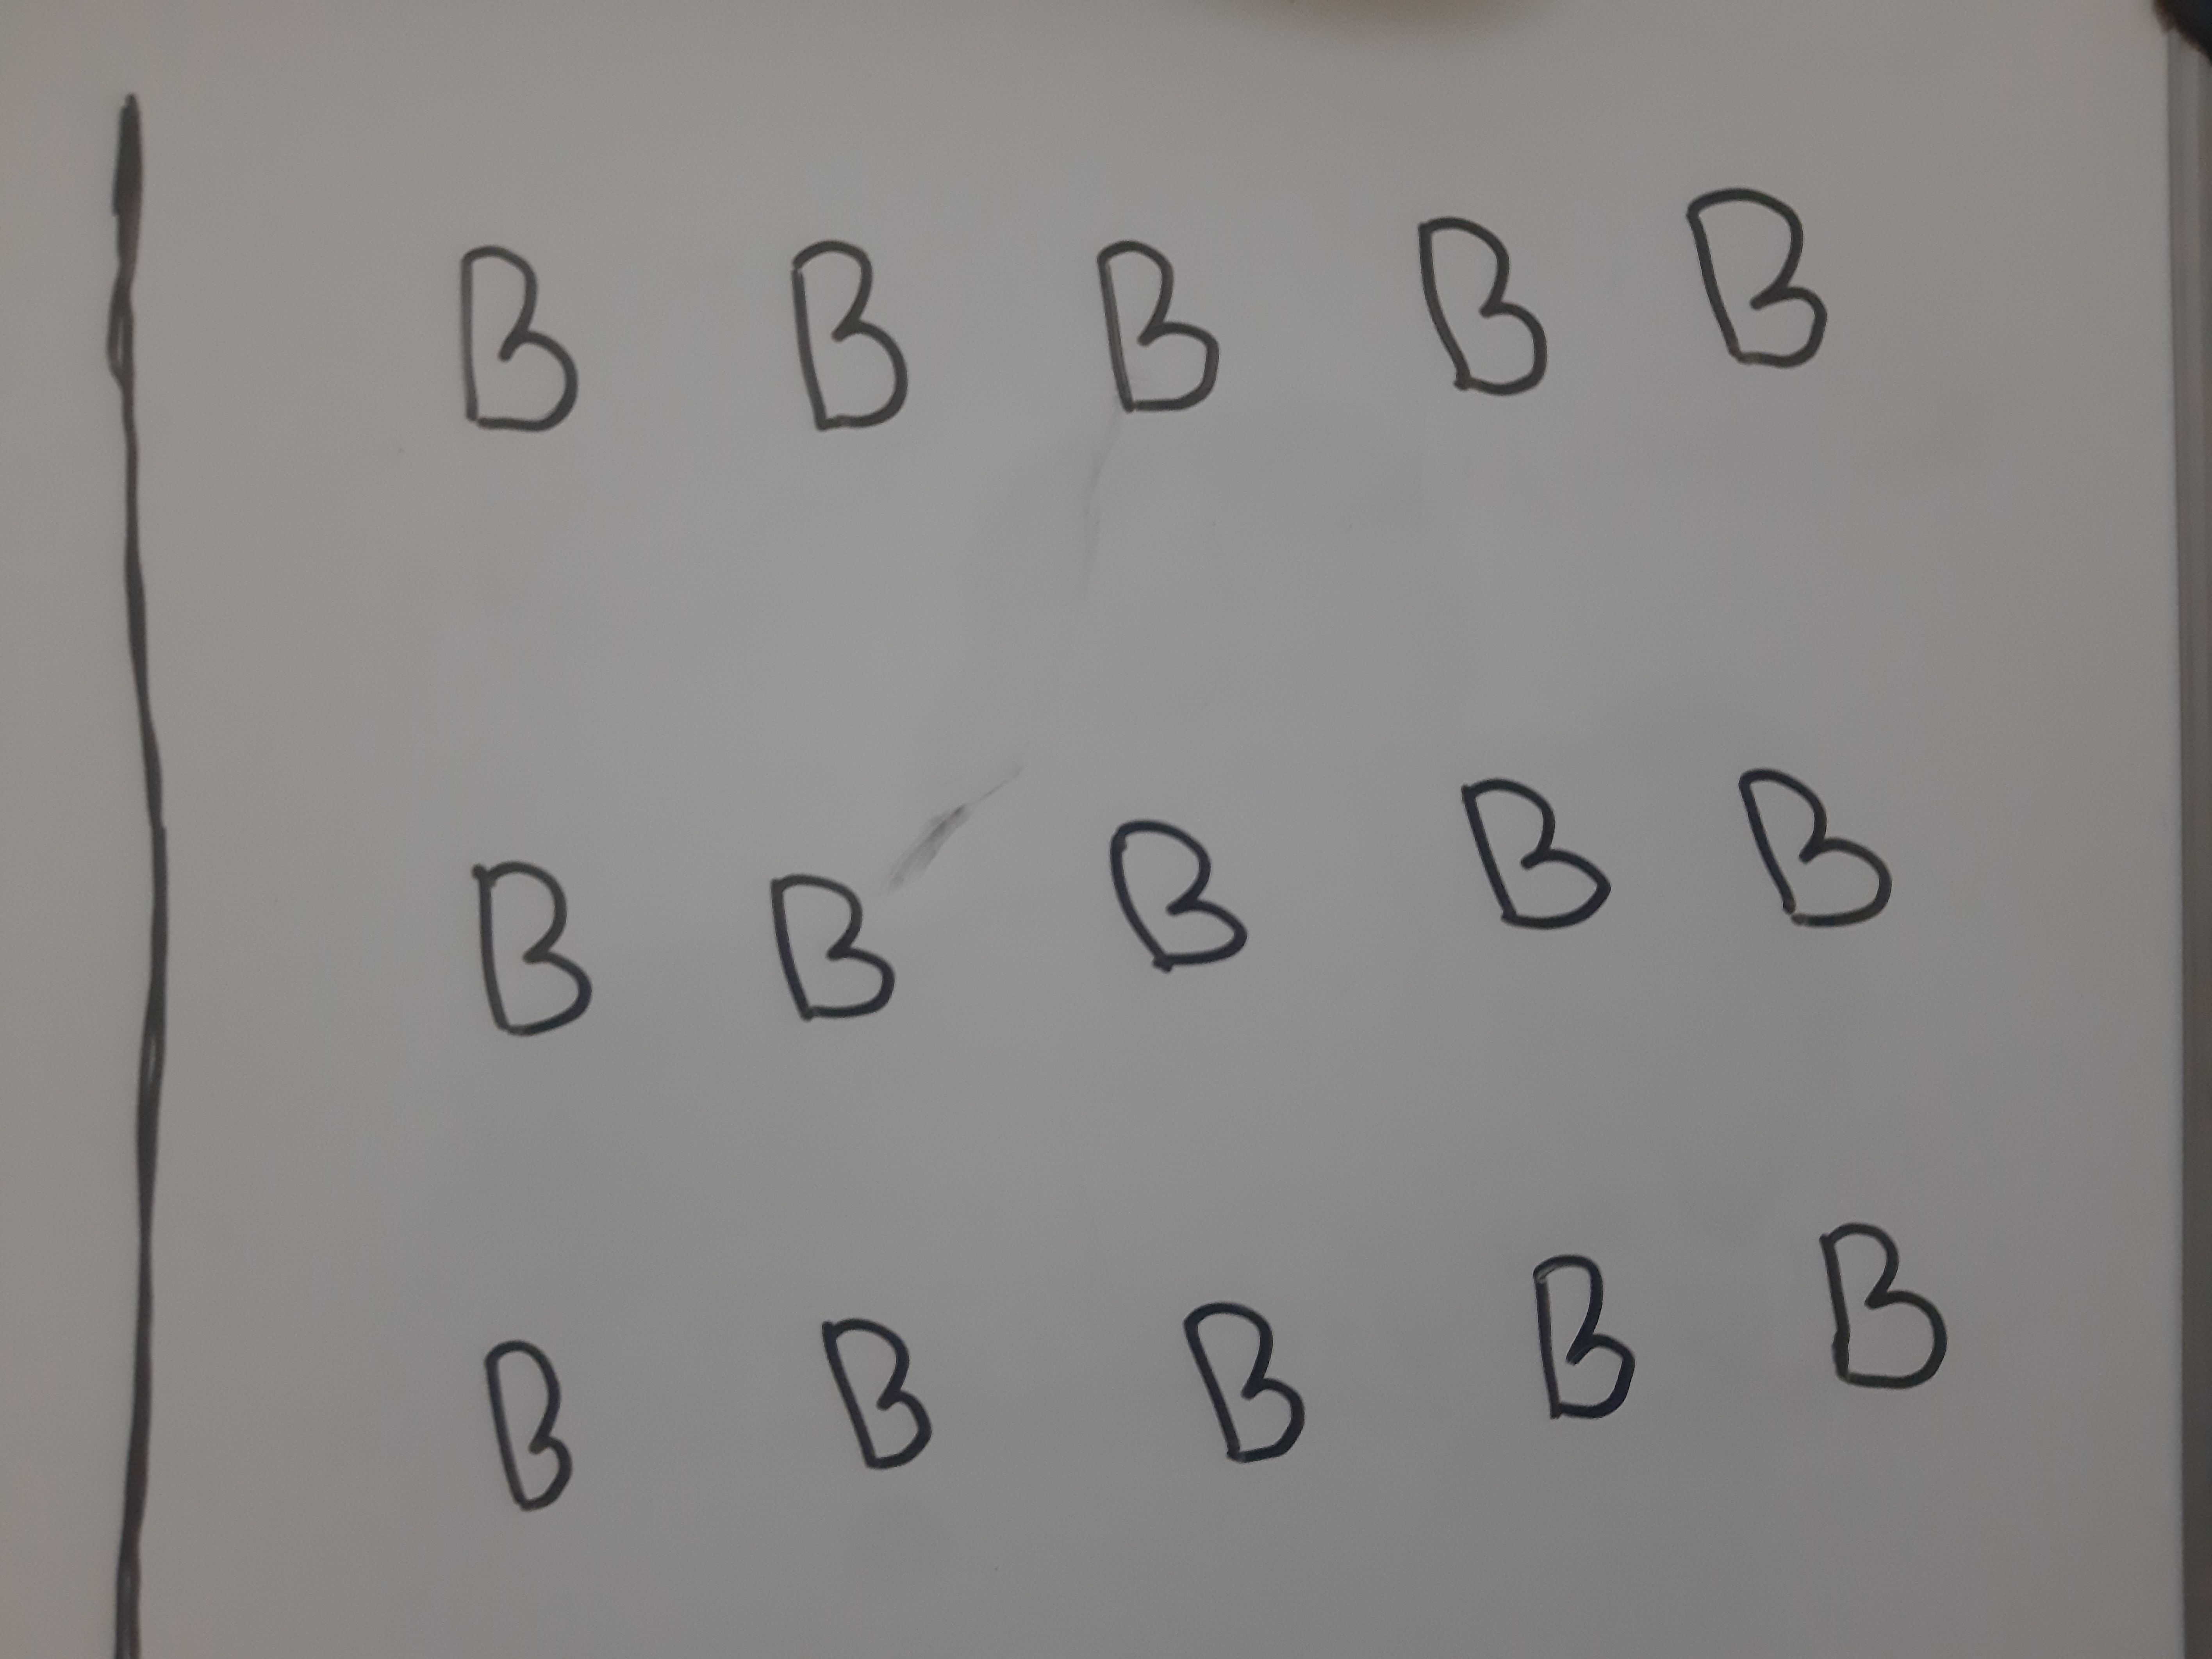
\includegraphics[width=.85\linewidth]{gambar/pengambilan_citra_depan.jpg}
    \caption{Pengambilan Citra dari Depan}
    \label{fig:citradepan}
  \end{subfigure}%
  \begin{subfigure}{.5\textwidth}
    \centering
    \captionsetup{width=.8\linewidth}
    \includegraphics[width=.85\linewidth]{gambar/pengambilan_citra_samping.jpg}
    \caption{Pengambilan Citra dari Samping}
    \label{fig:citrasamping}
  \end{subfigure}
  \caption{Pengambilan Citra dengan Variasi Sudut Pengambilan Gambar}
  \label{fig:pengambilancitrabervariasi}
\end{figure}

Secara spesifik, total persebaran citra pada masing-masing kelas dapat dilihat pada Tabel \ref{tb:citrapadatiapkelas} berikut. \par

% //FIXME: perbarui tabel
\begin{center}
  \begin{longtable}{|c|c|c|c|}
    \hline
    \textbf{Kelas} & \textbf{Jumlah Gambar} & \textbf{\textit{Train Sets}} & \textbf{\textit{Test Sets}} \\ \hline
      *                                    & 36                     & 29                  & 7                  \\ \hline
      =                                    & 50                     & 45                  & 5                  \\ \hline
      0                                    & 50                     & 45                  & 5                  \\ \hline
      1                                    & 50                     & 45                  & 5                  \\ \hline
      2                                    & 50                     & 45                  & 5                  \\ \hline
      3                                    & 50                     & 45                  & 5                  \\ \hline
      4                                    & 50                     & 45                  & 5                  \\ \hline
      5                                    & 50                     & 45                  & 5                  \\ \hline
      6                                    & 50                     & 45                  & 5                  \\ \hline
      7                                    & 50                     & 45                  & 5                  \\ \hline
      8                                    & 50                     & 45                  & 5                  \\ \hline
      9                                    & 50                     & 45                  & 5                  \\ \hline
      A                                    & 36                     & 29                  & 7                  \\ \hline
      B                                    & 30                     & 27                  & 3                  \\ \hline
      D                                    & 36                     & 29                  & 7                  \\ \hline
      E                                    & 36                     & 29                  & 7                  \\ \hline
      G                                    & 36                     & 29                  & 7                  \\ \hline
      H                                    & 36                     & 29                  & 7                  \\ \hline
      I                                    & 36                     & 29                  & 7                  \\ \hline
      J                                    & 36                     & 29                  & 7                  \\ \hline
      K                                    & 36                     & 29                  & 7                  \\ \hline
      L                                    & 36                     & 29                  & 7                  \\ \hline
      M                                    & 20                     & 16                  & 4                  \\ \hline
      N                                    & 20                     & 16                  & 4                  \\ \hline
      P                                    & 36                     & 29                  & 7                  \\ \hline
      R                                    & 36                     & 29                  & 7                  \\ \hline
      S                                    & 36                     & 29                  & 7                  \\ \hline
      T                                    & 36                     & 29                  & 7                  \\ \hline
      U                                    & 36                     & 29                  & 7                  \\ \hline
      V                                    & 36                     & 29                  & 7                  \\ \hline
      W                                    & 36                     & 29                  & 7                  \\ \hline 
    \caption{Jumlah Citra Pada Tiap Kelas}
    \label{tb:citrapadatiapkelas}
  \end{longtable}
\end{center}
  
\subsubsection{Hasil Proses Pelabelan Dataset}
\label{subsubsec:hasilpelabelan}

Proses pelabelan dilakukan dengan memberikan \textit{bounding box} pada tiap-tiap citra yang telah dikumpulkan pada tahap sebelumnya. Pada proses \textit{bounding box,} tiap-tiap citra yang termasuk sebagai objek dari tiap kelas dianotasi sehingga seluruh bagian objeknya berada didalam anotasi dan diberi label sesuai dengan kelas objeknya. Anotasi pada proses pelabelan ini menggunakan anotasi berbentuk segiempat. Setelah proses pelabelan dilakukan maka \textit{output} yang dihasilkan pada tiap citra yang diolah yaitu sebuah file citra yang sudah di-\textit{pre-process} dan sebuah file txt berisi titik koordinat dari tiap objek yang ada pada sebuah citra tersebut. Adapun proses pelabelan dataset dapat dilihat pada Gambar \ref{fig:labellingroboflow}. 

\begin{figure}[H]
  \centering
  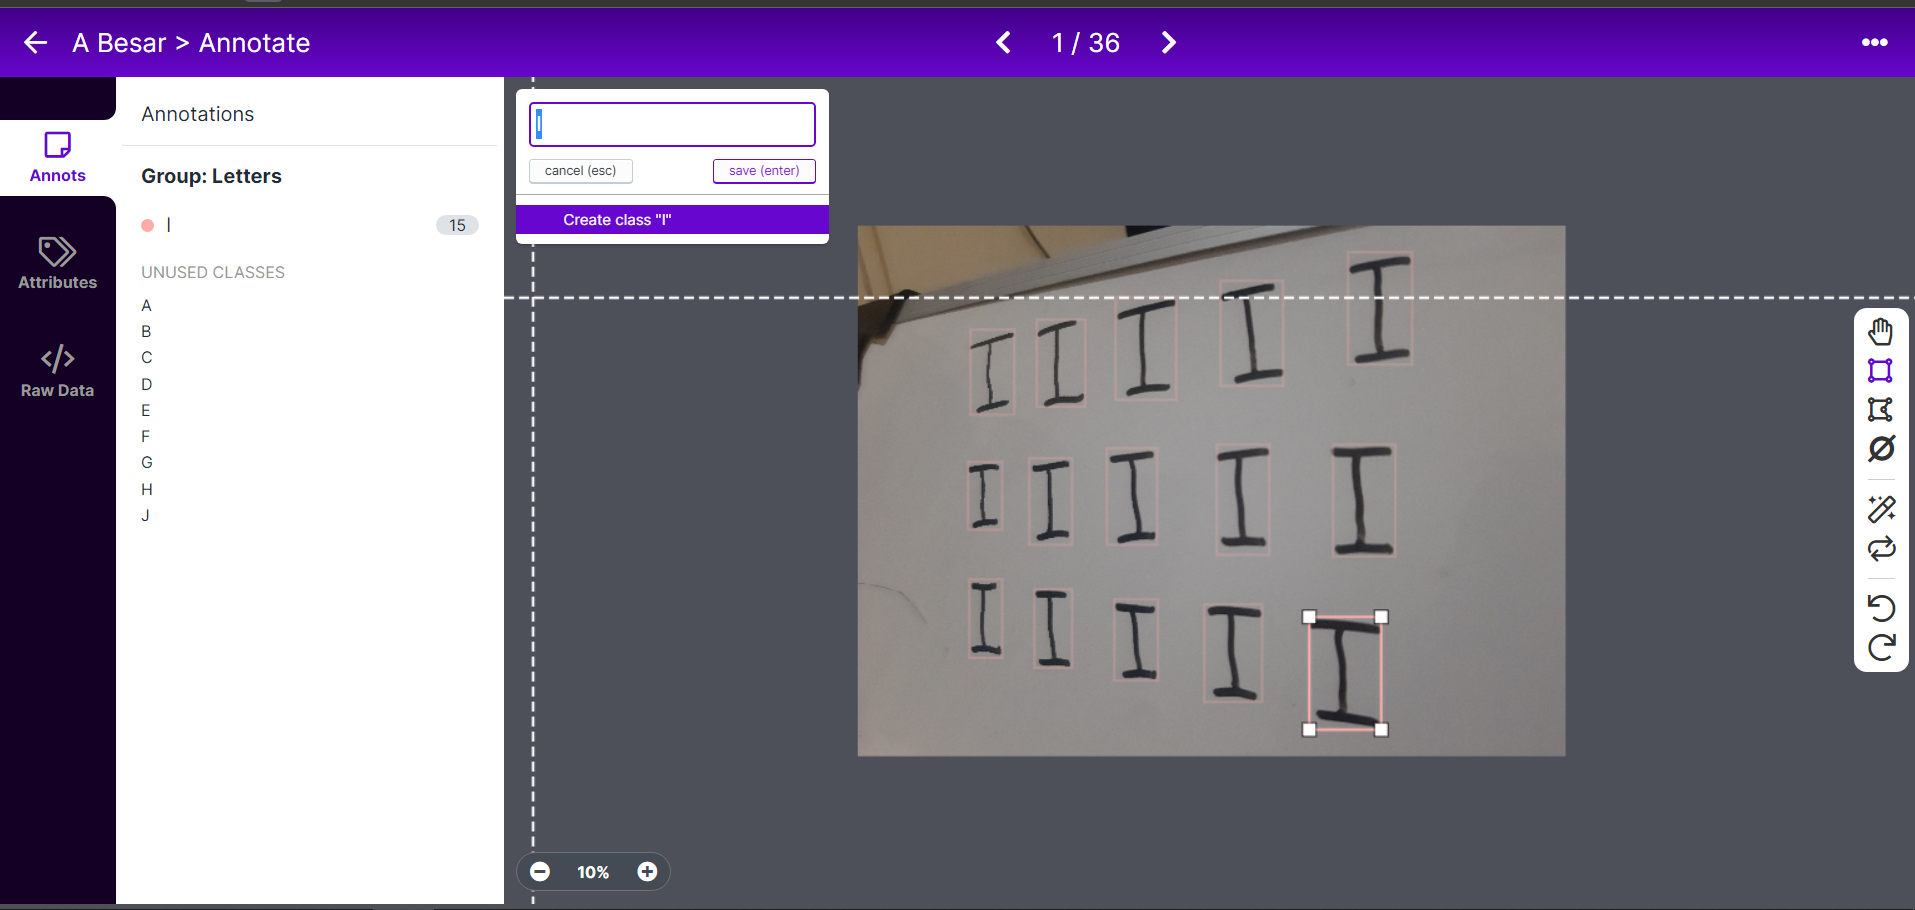
\includegraphics[scale=0.39]{gambar/labelling.png}
  \caption{Proses Pelabelan menggunakan Roboflow}
  \label{fig:labellingroboflow}
\end{figure}

Setelah dilakukan proses pelabelan, \textit{output} yang dihasilkan yaitu gambar yang memiliki \textit{bounding box}, dan apabila di-\textit{export} maka dataset hasil pelabelan terdiri dari 2 file yaitu file citra itu sendiri dan juga file txt yang berisi koordinat \textit{bounding box} yang ada pada suatu citra tersebut. Adapun total persebaran anotasi \textit{bounding box} pada masing-masing kelas dapat dilihat pada Tabel \ref{tb:anotasitiapkelas} berikut. 

% //FIXME: perbarui datanya
\begin{center}
  \begin{longtable}{|c|c|}
  \hline
  \textbf{Kelas} & \textbf{Jumlah Anotasi} \\ \hline
  A                                    & 540                     \\ \hline
  B                                    & 540                     \\ \hline
  C                                    & 540                     \\ \hline
  D                                    & 540                     \\ \hline
  E                                    & 900                     \\ \hline
  F                                    & 900                     \\ \hline
  G                                    & 540                     \\ \hline
  H                                    & 540                     \\ \hline
  I                                    & 540                     \\ \hline
  J                                    & 540                     \\ \hline
  K                                    & 540                     \\ \hline
  L                                    & 540                     \\ \hline
  M                                    & 900                     \\ \hline
  N                                    & 900                     \\ \hline
  O                                    & 540                     \\ \hline
  P                                    & 540                     \\ \hline
  Q                                    & 540                     \\ \hline
  R                                    & 540                     \\ \hline
  S                                    & 540                     \\ \hline
  T                                    & 540                     \\ \hline
  U                                    & 900                     \\ \hline
  V                                    & 900                     \\ \hline
  W                                    & 900                     \\ \hline
  X                                    & 540                     \\ \hline
  Y                                    & 540                     \\ \hline
  Z                                    & 540                     \\ \hline
  \caption{Jumlah Anotasi Pada Tiap Kelas}
  \label{tb:anotasitiapkelas}
  \end{longtable}
\end{center}
  

\subsubsection{Hasil \textit{Image Pre-Processing}}
\label{subsubsec:hasilpreprocess}

Pada tahap \textit{pre-process}, citra yang telah diberi label selanjutnya dilakukan \textit{pre-process} tertentu. Tahapan \textit{pre-process} bertujuan untuk mengurangi waktu \textit{training} dan meningkatkan performa. Secara ringkas, tahapan \textit{pre-process} yang dilakukan yaitu seperti pada Tabel \ref*{tb:checklistpreprocess}. Secara spesifik, pada tahapan \textit{pre-process} melakukan proses transformasi citra tertentu yaitu:
\begin{enumerate}[nolistsep]
% //TODO: pertimbangkan menggunakan noise pada preproses
  \item \textit{\textbf{Auto Orient.} Auto Orient} dilakukan untuk agar citra yang ditampilkan orientasinya sesuai dengan ketika diambil pada pengambilan awal.
  \item \textit{\textbf{Resize.} Resize} dilakukan untuk mengubah dimensi citra menjadi lebih kecil. Citra diubah dengan pengaturan \textit{stretch} sehingga tiap citra yang sebelumnya tidak memiliki dimensi ukuran 416x416 diregangkan ukurannya menjadi ukuran 416x416.
  \item \textit{\textbf{Grayscale.} \textnormal{Proses} Grayscale} bertujuan untuk memperkecil variasi warna gambar khususnya objek yang dibuat dengan spidol sehingga proses \textit{train} menjadi lebih cepat. Hasil dari proses \textit{grayscale} seperti pada Gambar \ref{fig:grayscallingdataset}.
    \begin{figure}[H]
      \centering
      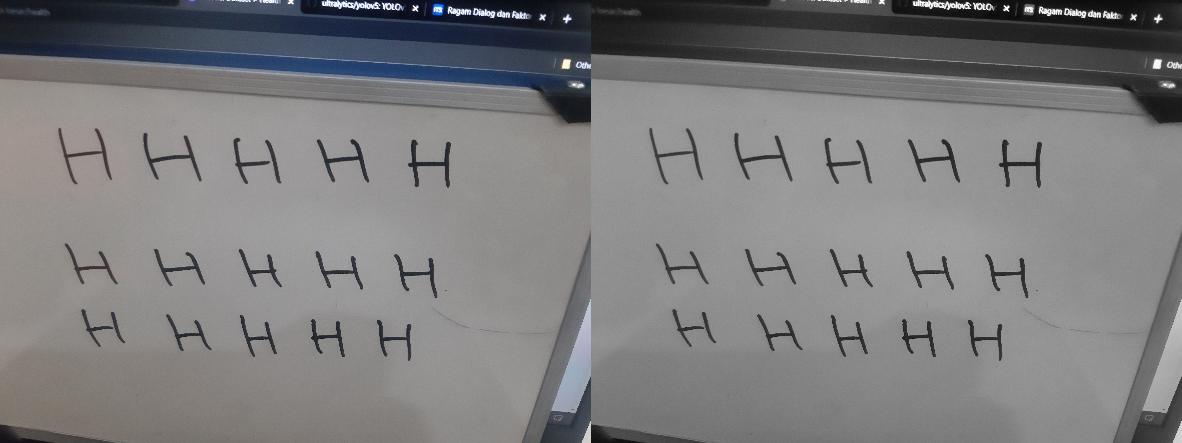
\includegraphics[scale=0.33]{gambar/grayscalling.png}
      \caption{Gambar Sebelum dan Setelah Proses \textit{Grayscalling}}
      \label{fig:grayscallingdataset}
    \end{figure}
  \item \textit{\textbf{Contrast.} Contrast} dilakukan agar tepian-tepian yang ada pada citra dapat lebih terlihat perbedaannya. Jenis \textit{contrast} yang dilakukan yaitu \textit{contrast stretching. Contrast stretching} adalah teknik transformasi citra yaitu meningkatkan kontras dalam citra dengan melakukan \textit{stretch} atau peregangan rentang intensitas nilai untuk menjangkau rentang nilai yang diinginkan.
  % \item \textit{\textbf{Filter Null.}}
  % \item \textit{\textbf{Blur.}}
  % \item \textit{\textbf{Noise.}}
  % \item \textit{\textbf{Bounding Box Rotation.}}
\end{enumerate}

\subsection{Hasil \textit{Training} dan \textit{Validation}}
\label{subsec:hasiltrainvaldata}

% halooooo, chesia was here
Pada tugas akhir ini, \textit{pretrained weight} yang digunakan yaitu YOLOv5s. \textit{pretrained weight} YOLOv5s dipilih karena jika dibandingkan dengan versi lain seperti YOLOv5m, YOLOv5l memiliki hasil yang relatif lebih rendah, namun dengan menggunakan YOLOv5s hasil dapat didapatkan lebih cepat dan juga cocok jika di-\textit{deploy} pada perangkat kecil seperti perangkat \textit{mobile}. Proses \textit{training} data dilakukan setelah proses pengumpulan citra, proses pelabelan, dan pre-proses gambar selesai dilaksanakan. Adapun hasil dari proses \textit{training} ini yaitu berupa model dan detail data angka pada tiap proses pengulangan  (epochs). Detail spesifikasi laptop yang digunakan dalam melakukan proses \textit{training} yaitu sesuai pada Tabel \ref{tb:spesifikasilaptop}, sedangkan detail hyperparameter dan konfigurasi yang digunakan dapat dilihat pada Tabel \ref*{tb:parametertrain} berikut. \par 

% //FIXME: perbarui tabel 
\begin{table}[H]
  \begin{center}
    \begin{tabularx}{0.5\textwidth}{|X<{\centering}|X<{\centering}|}
      \hline
      % \textbf{Parameter}                       & \textbf{Nilai}          \\ \hline
      \textit{Weights}                         & YOLOv5s                 \\ \hline
      \textit{Class Number}                    & 30                      \\ \hline
      Epochs                                   & 50                      \\ \hline
      \textit{Batch-Size}                      & 16                      \\ \hline
      \textit{Image Size}                      & 416                     \\ \hline
      \textit{Learning Rate}                   & 0.01                    \\ \hline
      \textit{Optimizer}                       & SGD                     \\ \hline
    \end{tabularx}
  \end{center}  
  \caption{Detail Hyperparameter yang Digunakan}
  \label{tb:parametertrain}
\end{table}


Proses \textit{training} dilakukan menggunakan dataset \textit{training set}. Setelah dilakukan proses \textit{train} dengan konfigurasi sesuai pada Tabel \ref*{tb:parametertrain}, selanjutnya dilakukan proses \textit{validation.} Pada tahapan \textit{validation} yaitu model diuji dengan menggunakan dataset \textit{validation set} dan kemudian didapatkan hasil \textit{train} berupa \textit{loss, precision, recall, \textnormal{dan} mAP} sesuai Gambar \ref*{fig:trainresult} yaitu: \par

% //FIXME: perbarui tabel
\begin{figure}[H]
  \centering
  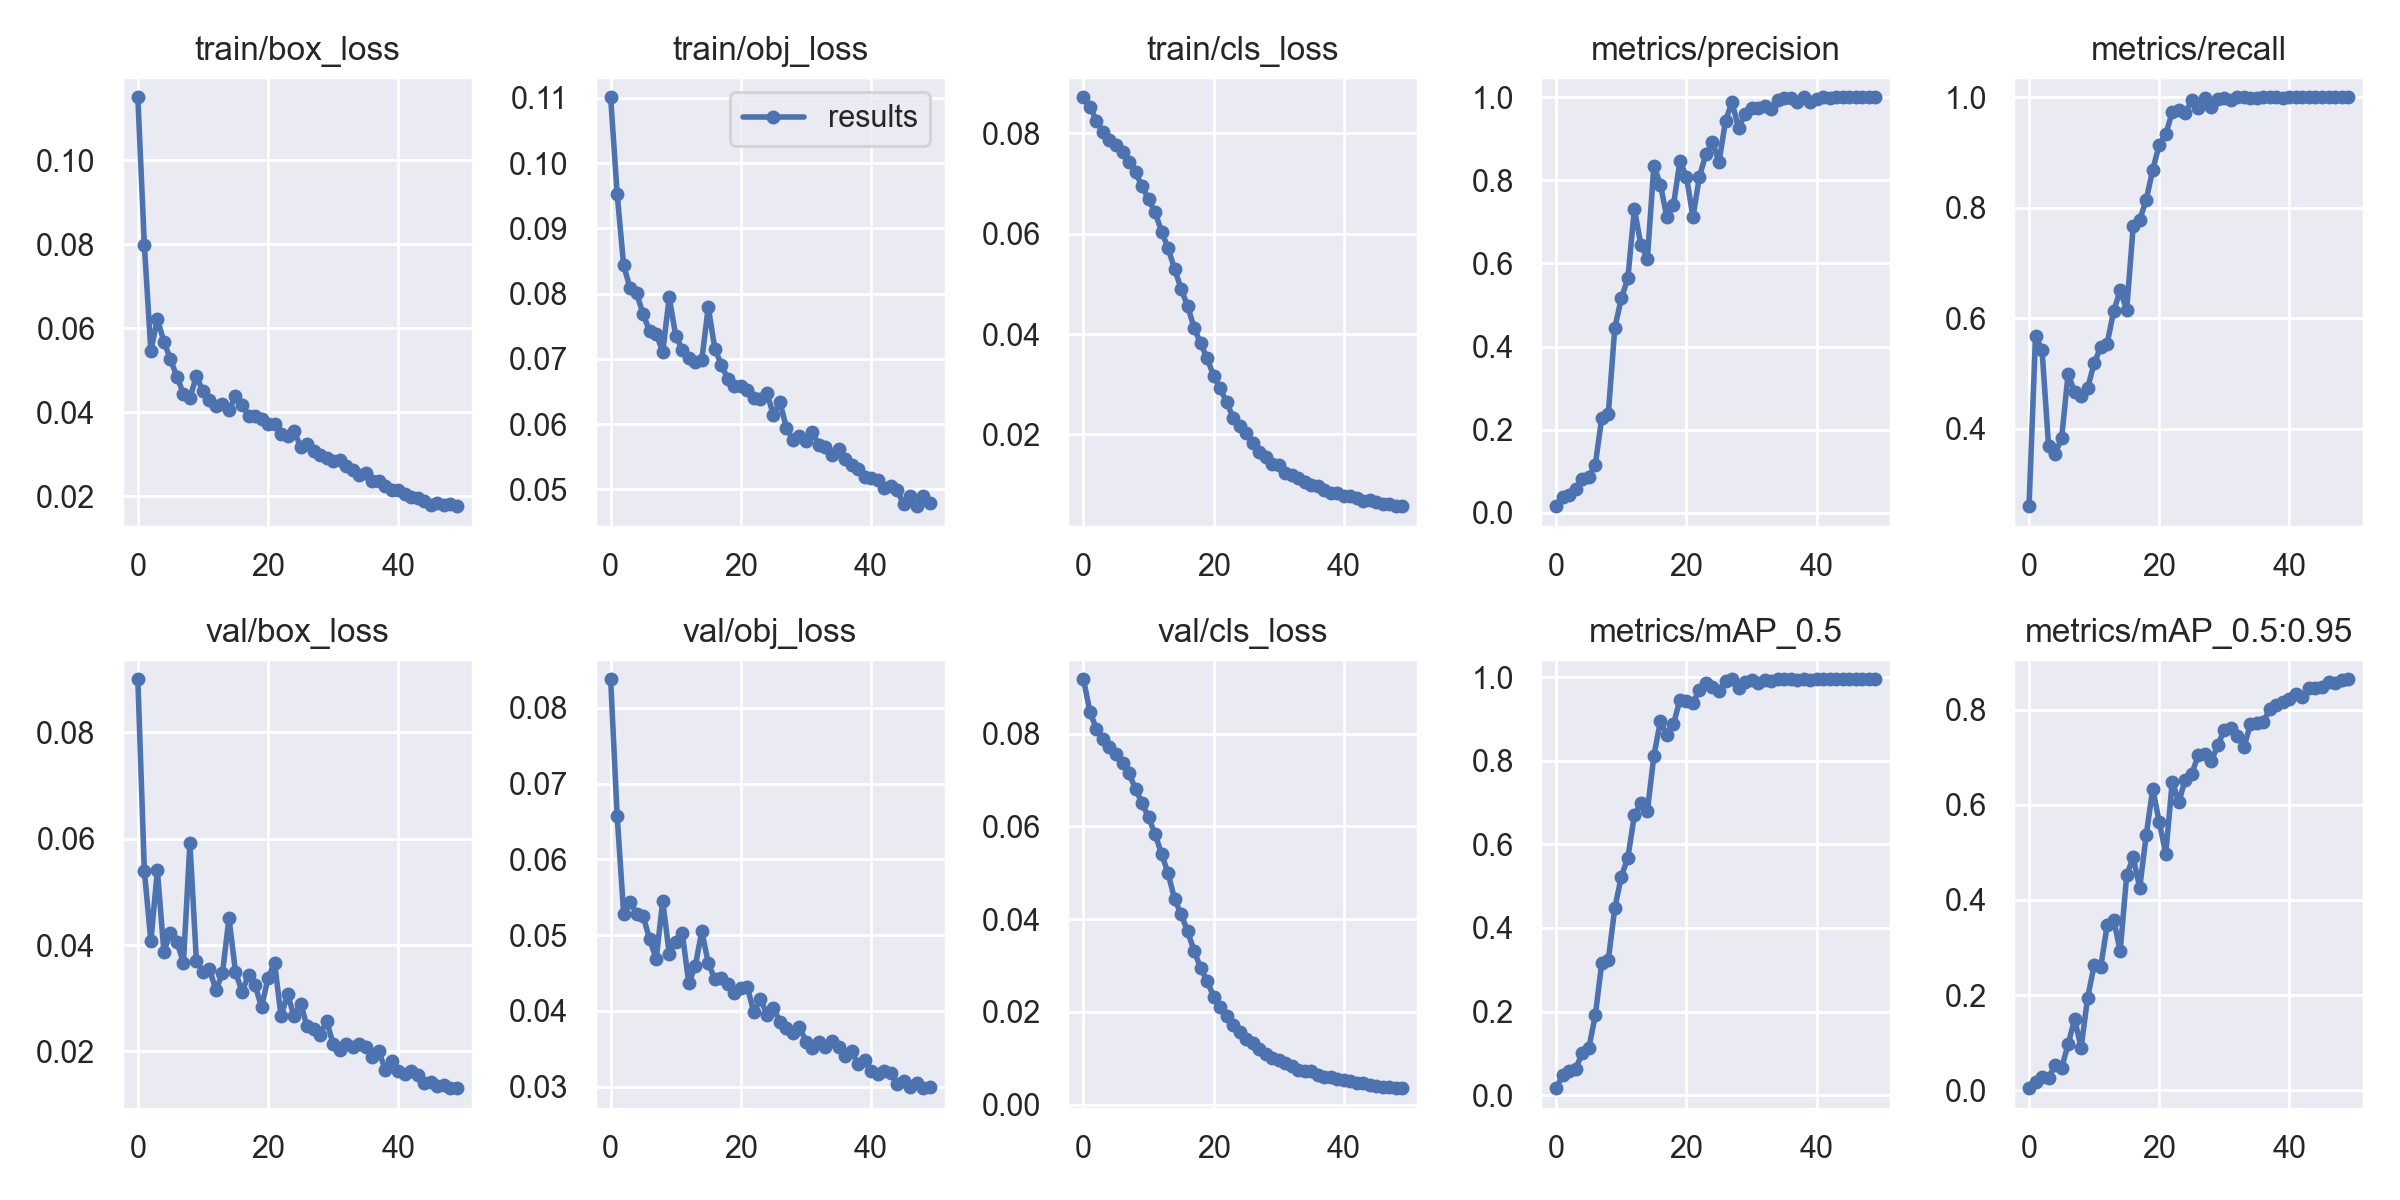
\includegraphics[scale=0.5]{gambar/train_result.png}
  \caption{Hasil Training menggunakan YOLOv5s}
  \label{fig:trainresult}
\end{figure}

\noindent Serta didapatkan detail dari akurasi masing-masing huruf yaitu sebagai berikut: \par

% //FIXME: perbarui tabel
\begin{center}
  \begin{longtable}[c]{|c|c|c|c|c|c|c|}
    \hline
    \textbf{Kelas} & \textbf{Gambar} & \textbf{Jumlah Label} & \textbf{P} & \textbf{R} & \textbf{mAP 0.5} & \textbf{mAP 0.5 0.95} \\ \hline
    \endfirsthead
    %
    \endhead
    %
    *              & 7                          & 105                   & 0.999      & 1          & 0.995            & 0.875                 \\ \hline
    =              & 7                          & 105                   & 0.999      & 1          & 0.995            & 0.907                 \\ \hline
    0              & 7                          & 105                   & 0.999      & 1          & 0.995            & 0.773                 \\ \hline
    1              & 7                          & 105                   & 0.999      & 1          & 0.995            & 0.83                  \\ \hline
    2              & 11                         & 165                   & 1          & 1          & 0.995            & 0.849                 \\ \hline
    3              & 11                         & 165                   & 0.999      & 1          & 0.995            & 0.854                 \\ \hline
    4              & 7                          & 105                   & 0.999      & 1          & 0.995            & 0.895                 \\ \hline
    5              & 7                          & 105                   & 0.999      & 1          & 0.995            & 0.872                 \\ \hline
    6              & 7                          & 105                   & 0.999      & 1          & 0.995            & 0.862                 \\ \hline
    7              & 7                          & 105                   & 1          & 1          & 0.995            & 0.875                 \\ \hline
    8              & 7                          & 105                   & 0.999      & 1          & 0.995            & 0.845                 \\ \hline
    9              & 7                          & 105                   & 0.999      & 1          & 0.995            & 0.859                 \\ \hline
    A              & 7                          & 105                   & 0.999      & 1          & 0.995            & 0.875                 \\ \hline
    B              & 7                          & 105                   & 0.999      & 1          & 0.995            & 0.907                 \\ \hline
    D              & 7                          & 105                   & 0.999      & 1          & 0.995            & 0.83                  \\ \hline
    E              & 11                         & 165                   & 1          & 1          & 0.995            & 0.849                 \\ \hline
    G              & 7                          & 105                   & 0.999      & 1          & 0.995            & 0.895                 \\ \hline
    H              & 7                          & 105                   & 0.999      & 1          & 0.995            & 0.872                 \\ \hline
    I              & 7                          & 105                   & 0.999      & 1          & 0.995            & 0.862                 \\ \hline
    J              & 7                          & 105                   & 1          & 1          & 0.995            & 0.875                 \\ \hline
    K              & 7                          & 105                   & 0.999      & 1          & 0.995            & 0.845                 \\ \hline
    L              & 7                          & 105                   & 0.999      & 1          & 0.995            & 0.859                 \\ \hline
    M              & 11                         & 165                   & 1          & 1          & 0.995            & 0.832                 \\ \hline
    N              & 11                         & 165                   & 1          & 1          & 0.995            & 0.799                 \\ \hline
    P              & 7                          & 105                   & 1          & 1          & 0.995            & 0.824                 \\ \hline
    R              & 7                          & 105                   & 1          & 1          & 0.995            & 0.844                 \\ \hline
    S              & 7                          & 105                   & 1          & 1          & 0.995            & 0.893                 \\ \hline
    T              & 7                          & 105                   & 0.999      & 1          & 0.995            & 0.874                 \\ \hline
    U              & 11                         & 165                   & 0.999      & 1          & 0.995            & 0.844                 \\ \hline
    V              & 11                         & 165                   & 0.999      & 1          & 0.995            & 0.867                 \\ \hline
    W              & 11                         & 165                   & 0.999      & 1          & 0.995            & 0.854                 \\ \hline
    \caption{Hasil Training Perkelas}
    \label{tb:trainperkelas}
  \end{longtable}
\end{center}

% //FIXME: lengkapi berdasarkan data model
Setelah didapatkan hasil model, dilakukan proses pengujian untuk menentukan apakah model tersebut sudah cukup akurat atau masih membutuhkan perbaikan. Pada proses pengujian didapatkan hasil bahwa model 
sementara masih \textit{\textbf{overfit}} dikarenakan walaupun pada hasil \textit{training} memiliki akurasi cukup tinggi, namun ketika dilakukan uji coba menggunakan gambar diluar dataset yag telah disediakan hasilnya masih berantakan. \par
% sudah dapat berfungsi seperti ditunjukkan pada gambar berikut. \par
% //TODO: tambah gambar pas detect model

% \subsection{Hasil \textit{Validation}}
% \label{subsec:hasilvalidation}

\subsection{Hasil Pembuatan Algoritma Konversi Gambar menjadi Teks}
\label{subsec:hasilmembangunmodel}

% //FIXME: lengkapi dengan hasil model
Setelah didapatkan model hasil \textit{training} dan sudah memiliki akurasi cukup untuk dapat melakukan deteksi dengan baik, selanjutnya dilakukan proses pembangunan model konversi gambar menjadi teks. Proses pembangunan model konversi gambar menjadi teks ini diprogram dengan menggunakan bahasa Python. Adapun alur model konversi gambar menjadi teks dimlai dari pengguna melakukan \textit{input} gambar yang ingin dikonversi kedalam program. Setelah gambar dimasukkan kedalam program, gambar tersebut diubah ukurannya menjadi (...), dengan menggunakan \textit{library} opencv. \par

Setelah ukuran gambar disesuaikan, selanjutnya menentukan koordinat seluruh \textit{bounding box} yang tersedia dan terbaca dengan menggunakan model yang telah di\textit{-train} sebelumnya. Setelah koordinat \textit{bounding box} didapat, seluruh \textit{bounding box} yang terbaca dikelompokan berdasarkan jarak antara \textit{bounding box} pertama dengan \textit{bounding box} selanjutnya, jika jarak antaranya memenuhi \textit{threshold} tertentu, maka akan dikelompokan kedalam sebuah List yang sama, dan jika tidak memenuhi maka akan diletakan pada kelompok List berikutnya. Adapun \textit{threshold} yang digunakan yaitu pada koordinat X sebesar (...) dan koordinat Y sebesar (...). Prioritas pengelompokan diatur berdasarkan koordinat Y terlebih dahulu kemudian dilanjutkan dengan koordinat X, hal ini bertujuan agar teks yang ditampilkan berurutan dari baris paling atas lalu bergerak kearah X+ (kanan), dan dilanjut pada baris kedua dan seterusnya. \par

Ketika seluruh \textit{bounding box} telah disortir dan dikelompokkan berdasarkan koordinat X dan Y, proses selanjutnya yaitu seluruh \textit{bounding box} dikembalikan nilainya. Adapun nilai kembalian yang didapatkan dapat ditampilkan dalam gambar langsung ataupun dalam bentuk String. 

\section{Skenario Pengujian}
\label{sec:skenariopengujian}

Pada sub ini dilakukan berbagai skenario pengujian guna mengetahui tingkat kesalahan dan membuka potensi pengembangan penelitian dimasa mendatang serta menarik kesimpulan secara keseluruhan. Secara spesifik, skenario pengujian yang dilakukan yaitu sebagai berikut: \par

\subsection{Pengujian Menggunakan \textit{Pretrained Weight} Model yang Bervariasi}
\label{subsec:pengujianpretrainedweight}

Pada pengujian pertama yaitu pengujian menggunakan \textit{pretrained weight} model yang bervariasi. Tujuan dari pengujian ini yaitu untuk membandingkan performa dan hasil yang didapat dengan performa dan hasil yang didapat dari model lain. Pada pengujian dengan \textit{pretrained weight} model ini menggunakan model YOLOv5n, YOLOv5s, dan YOLOv5m. Pengujian dilaksanakan dengan cara melakukan proses \textit{train} dengan konfigurasi serupa antar parameter dan \textit{hyperparameter.} Pada tiap \textit{pretrained weight} model yang diuji prosesnya diulang sebanyak 2 kali. Dari pengujian pertama ini didapatkan hasil seperti pada Tabel \ref*{tb:variasipretrainedweight} berikut. \par

\begin{center}
  \begin{longtable}[c]{|c|cc|cc|cc|}
    \hline
    \multirow{2}{*}{\textbf{}}                                                         & \multicolumn{2}{c|}{\textbf{YOLOv5n}}  & \multicolumn{2}{c|}{\textbf{YOLOv5s}}  & \multicolumn{2}{c|}{\textbf{YOLOv5m}}  \\ \cline{2-7} 
                                                                                      & \multicolumn{1}{c|}{1}       & 2       & \multicolumn{1}{c|}{1}       & 2       & \multicolumn{1}{c|}{1}       & 2       \\ \hline
    \endfirsthead
    %
    \endhead
    %
    \textit{\textbf{\begin{tabular}[c]{@{}c@{}}Training\\ Box Loss\end{tabular}}}      & \multicolumn{1}{c|}{not yet} & not yet & \multicolumn{1}{c|}{not yet} & not yet & \multicolumn{1}{c|}{not yet} & not yet \\ \hline
    \textit{\textbf{\begin{tabular}[c]{@{}c@{}}Training\\ Object Loss\end{tabular}}}   & \multicolumn{1}{c|}{not yet} & not yet & \multicolumn{1}{c|}{not yet} & not yet & \multicolumn{1}{c|}{not yet} & not yet \\ \hline
    \textit{\textbf{\begin{tabular}[c]{@{}c@{}}Training\\ Class Loss\end{tabular}}}    & \multicolumn{1}{c|}{not yet} & not yet & \multicolumn{1}{c|}{not yet} & not yet & \multicolumn{1}{c|}{not yet} & not yet \\ \hline
    \textit{\textbf{\begin{tabular}[c]{@{}c@{}}Validation\\ Box Loss\end{tabular}}}    & \multicolumn{1}{c|}{not yet} & not yet & \multicolumn{1}{c|}{not yet} & not yet & \multicolumn{1}{c|}{not yet} & not yet \\ \hline
    \textit{\textbf{\begin{tabular}[c]{@{}c@{}}Validation\\ Object Loss\end{tabular}}} & \multicolumn{1}{c|}{not yet} & not yet & \multicolumn{1}{c|}{not yet} & not yet & \multicolumn{1}{c|}{not yet} & not yet \\ \hline
    \textit{\textbf{\begin{tabular}[c]{@{}c@{}}Validation\\ Class Loss\end{tabular}}}  & \multicolumn{1}{c|}{not yet} & not yet & \multicolumn{1}{c|}{not yet} & not yet & \multicolumn{1}{c|}{not yet} & not yet \\ \hline
    \multicolumn{1}{|l|}{\textit{\textbf{Precision}}}                                  & \multicolumn{1}{c|}{not yet} & not yet & \multicolumn{1}{c|}{not yet} & not yet & \multicolumn{1}{c|}{not yet} & not yet \\ \hline
    \multicolumn{1}{|l|}{\textit{\textbf{Recall}}}                                     & \multicolumn{1}{c|}{not yet} & not yet & \multicolumn{1}{c|}{not yet} & not yet & \multicolumn{1}{c|}{not yet} & not yet \\ \hline
    \multicolumn{1}{|l|}{\textbf{mAP}}                                                 & \multicolumn{1}{c|}{not yet} & not yet & \multicolumn{1}{c|}{not yet} & not yet & \multicolumn{1}{c|}{not yet} & not yet \\ \hline
    \caption{Pengujian dengan Variasi Pretrained Weight }
    \label{tb:variasipretrainedweight}\\
  \end{longtable}
\end{center}

% //TODO: tambahin grafik dari tiap training dan tiap jenis model
% Dari tabel berikut dapat terlihat bahwa nilai \textit{loss} terendah yaitu pada model (...) dan nilai precision tertinggi yaitu pada model (...).

\subsection{Pengujian Menggunakan \textit{Input} Citra Tulisan dari Responden Berbeda}
\label{subsec:pengujiancitrabedapenulis}

Pada pengujian kedua yaitu pengujian menggunakan \textit{input} citra tulisan dari penulis berbeda. Tujuan dari pengujian ini yaitu untuk mengetahui akurasi model ketika dihadapkan dengan tulisan dari penulis lain. Hal tersebut diperlukan karena pada proses pembuatan dataset, dataset dibuat berdasarkan gaya penulisan dari 1 orang saja. Pada tahap pengujian ini, penulis meminta responden untuk menuliskan kalimat tertentu kepada beberapa responden dan mengambil citra dari tulisan tersebut untuk kemudian diberikan kepada model. Adapun tulisan yang diberikan sama antar responden dan juga sudut serta jarak pengambilan citra juga disamakan. Perbandingan hasil pembacaan model terhadap citra tulisan dari responden berbeda didapatkan hasil yaitu sebagai berikut.
% //TODO: citra dari 5 orang berbeda

\subsection{Pengujian Menggunakan \textit{Input} Citra dengan Jarak Pengambilan Citra Bervariasi}
\label{subsec:pengujiancitrabedajarak}

Pada pengujian ketiga yaitu pengujian menggunakan \textit{input} citra dengan jarak pengambilan citra yang bervariasi. Tujuan dari pengujian ini yaitu untuk mengetahui akurasi model ketika citra yang akan diberikan diambil dari jarak pengambilan gambar yang berbeda, serta untuk mengetahui pengaruh jarak pengambilan citra dengan performa dari model. Hal tersebut diperlukan karena pada kondisi nyata tidak menutup kemungkinan bahwa citra yang diberikan diambil dari jarak yang cukup jauh ataupun cukup dekat. Adapun pada pengujian kali ini, variasi yang digunakan yaitu pengambilan citra pada jarak kisaran 20cm, kisaran 30cm, dan kisaran 40cm. Perbandingan hasil pembacaan model terhadap citra tulisan dari jarak pengambilan bervariasi didapatkan hasil yaitu seperti pada Gambar \ref*{fig:citra20cm}, Gambar \ref*{fig:citra30cm}, dan Gambar \ref*{fig:citra40cm} berikut.

% //FIXME: ganti gambar, versi terang dari 2 konten isi berbeda (sama penulis, beda konten)
% 20cm
\begin{figure}[H]
  \begin{subfigure}{.5\textwidth}
    \centering
    \captionsetup{width=.8\linewidth}
    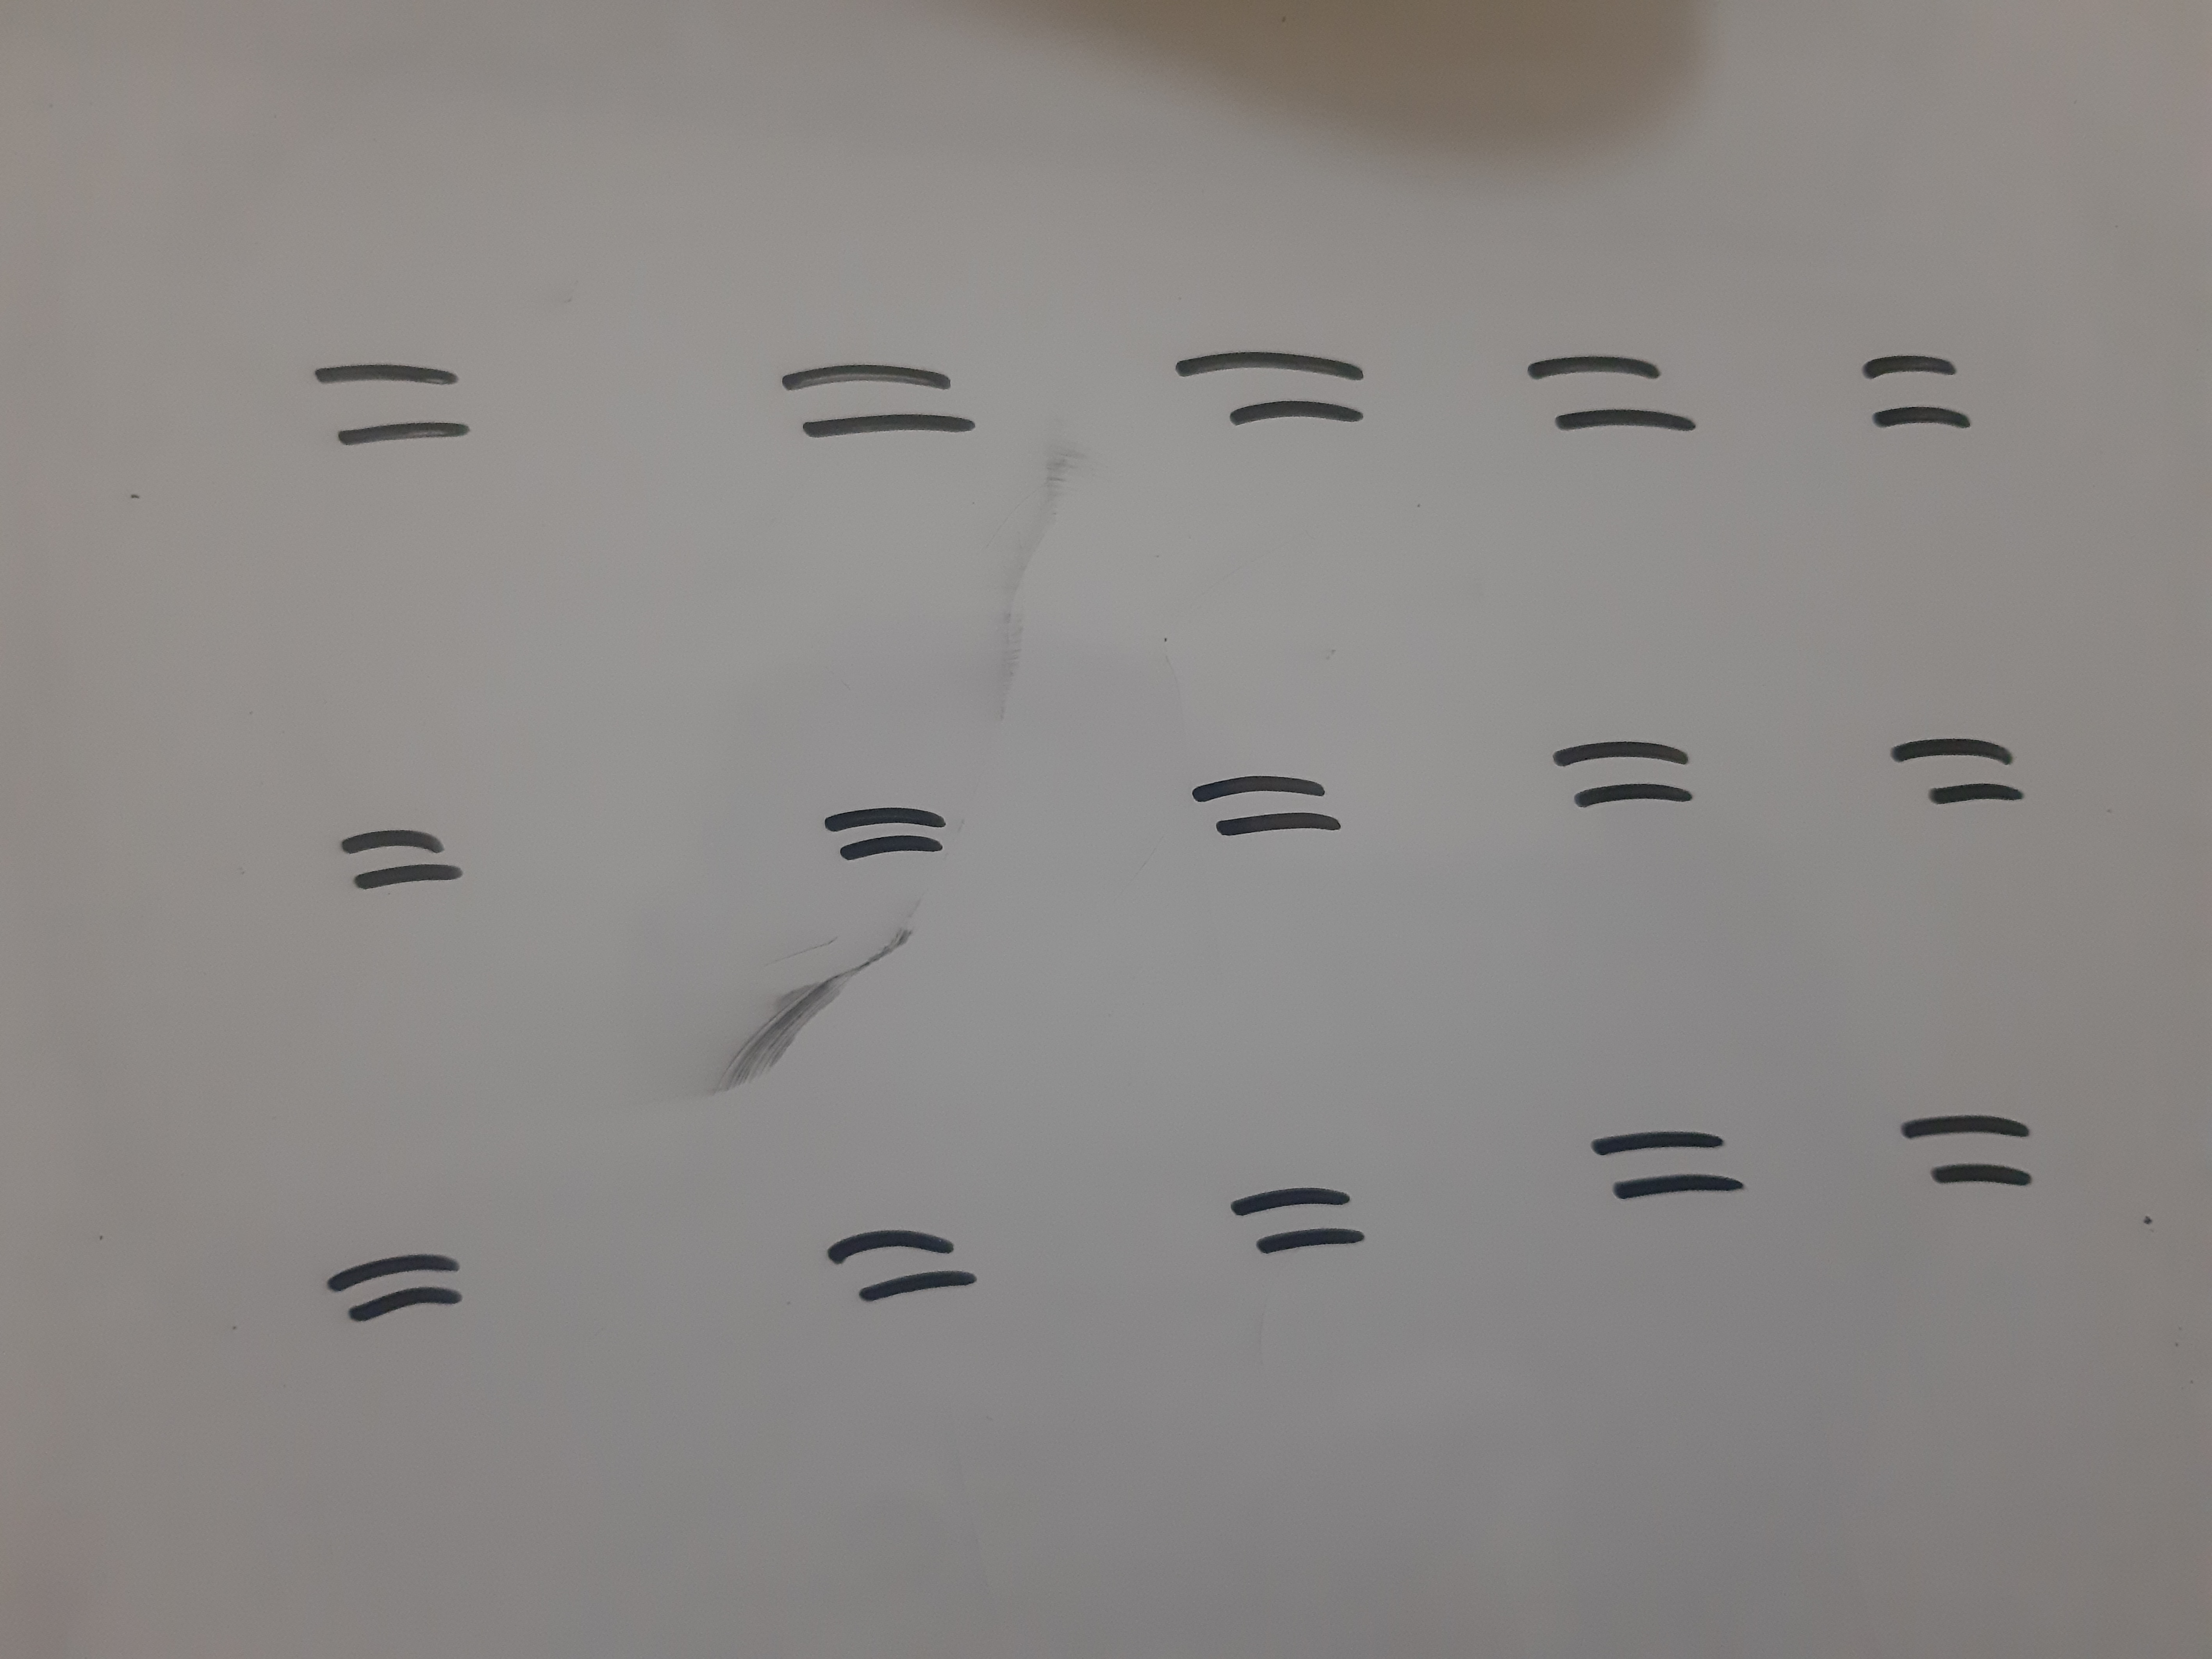
\includegraphics[width=.85\linewidth]{gambar/pengambilan_citra_terang.jpg}
    \caption{Sampel 1, Pengambilan Citra Jarak 20 Cm}
    \label{fig:citra120cm}
  \end{subfigure}%
  \begin{subfigure}{.5\textwidth}
    \centering
    \captionsetup{width=.8\linewidth}
    \includegraphics[width=.85\linewidth]{gambar/pengambilan_citra_gelap.jpg}
    \caption{Sampel 2, Pengambilan Citra Jarak 20 Cm}
    \label{fig:citra220cm}
  \end{subfigure}
  \caption{Pengambilan Citra Jarak 20 Cm}
  \label{fig:citra20cm}
\end{figure}

% 30cm
\begin{figure}[H]
  \begin{subfigure}{.5\textwidth}
    \centering
    \captionsetup{width=.8\linewidth}
    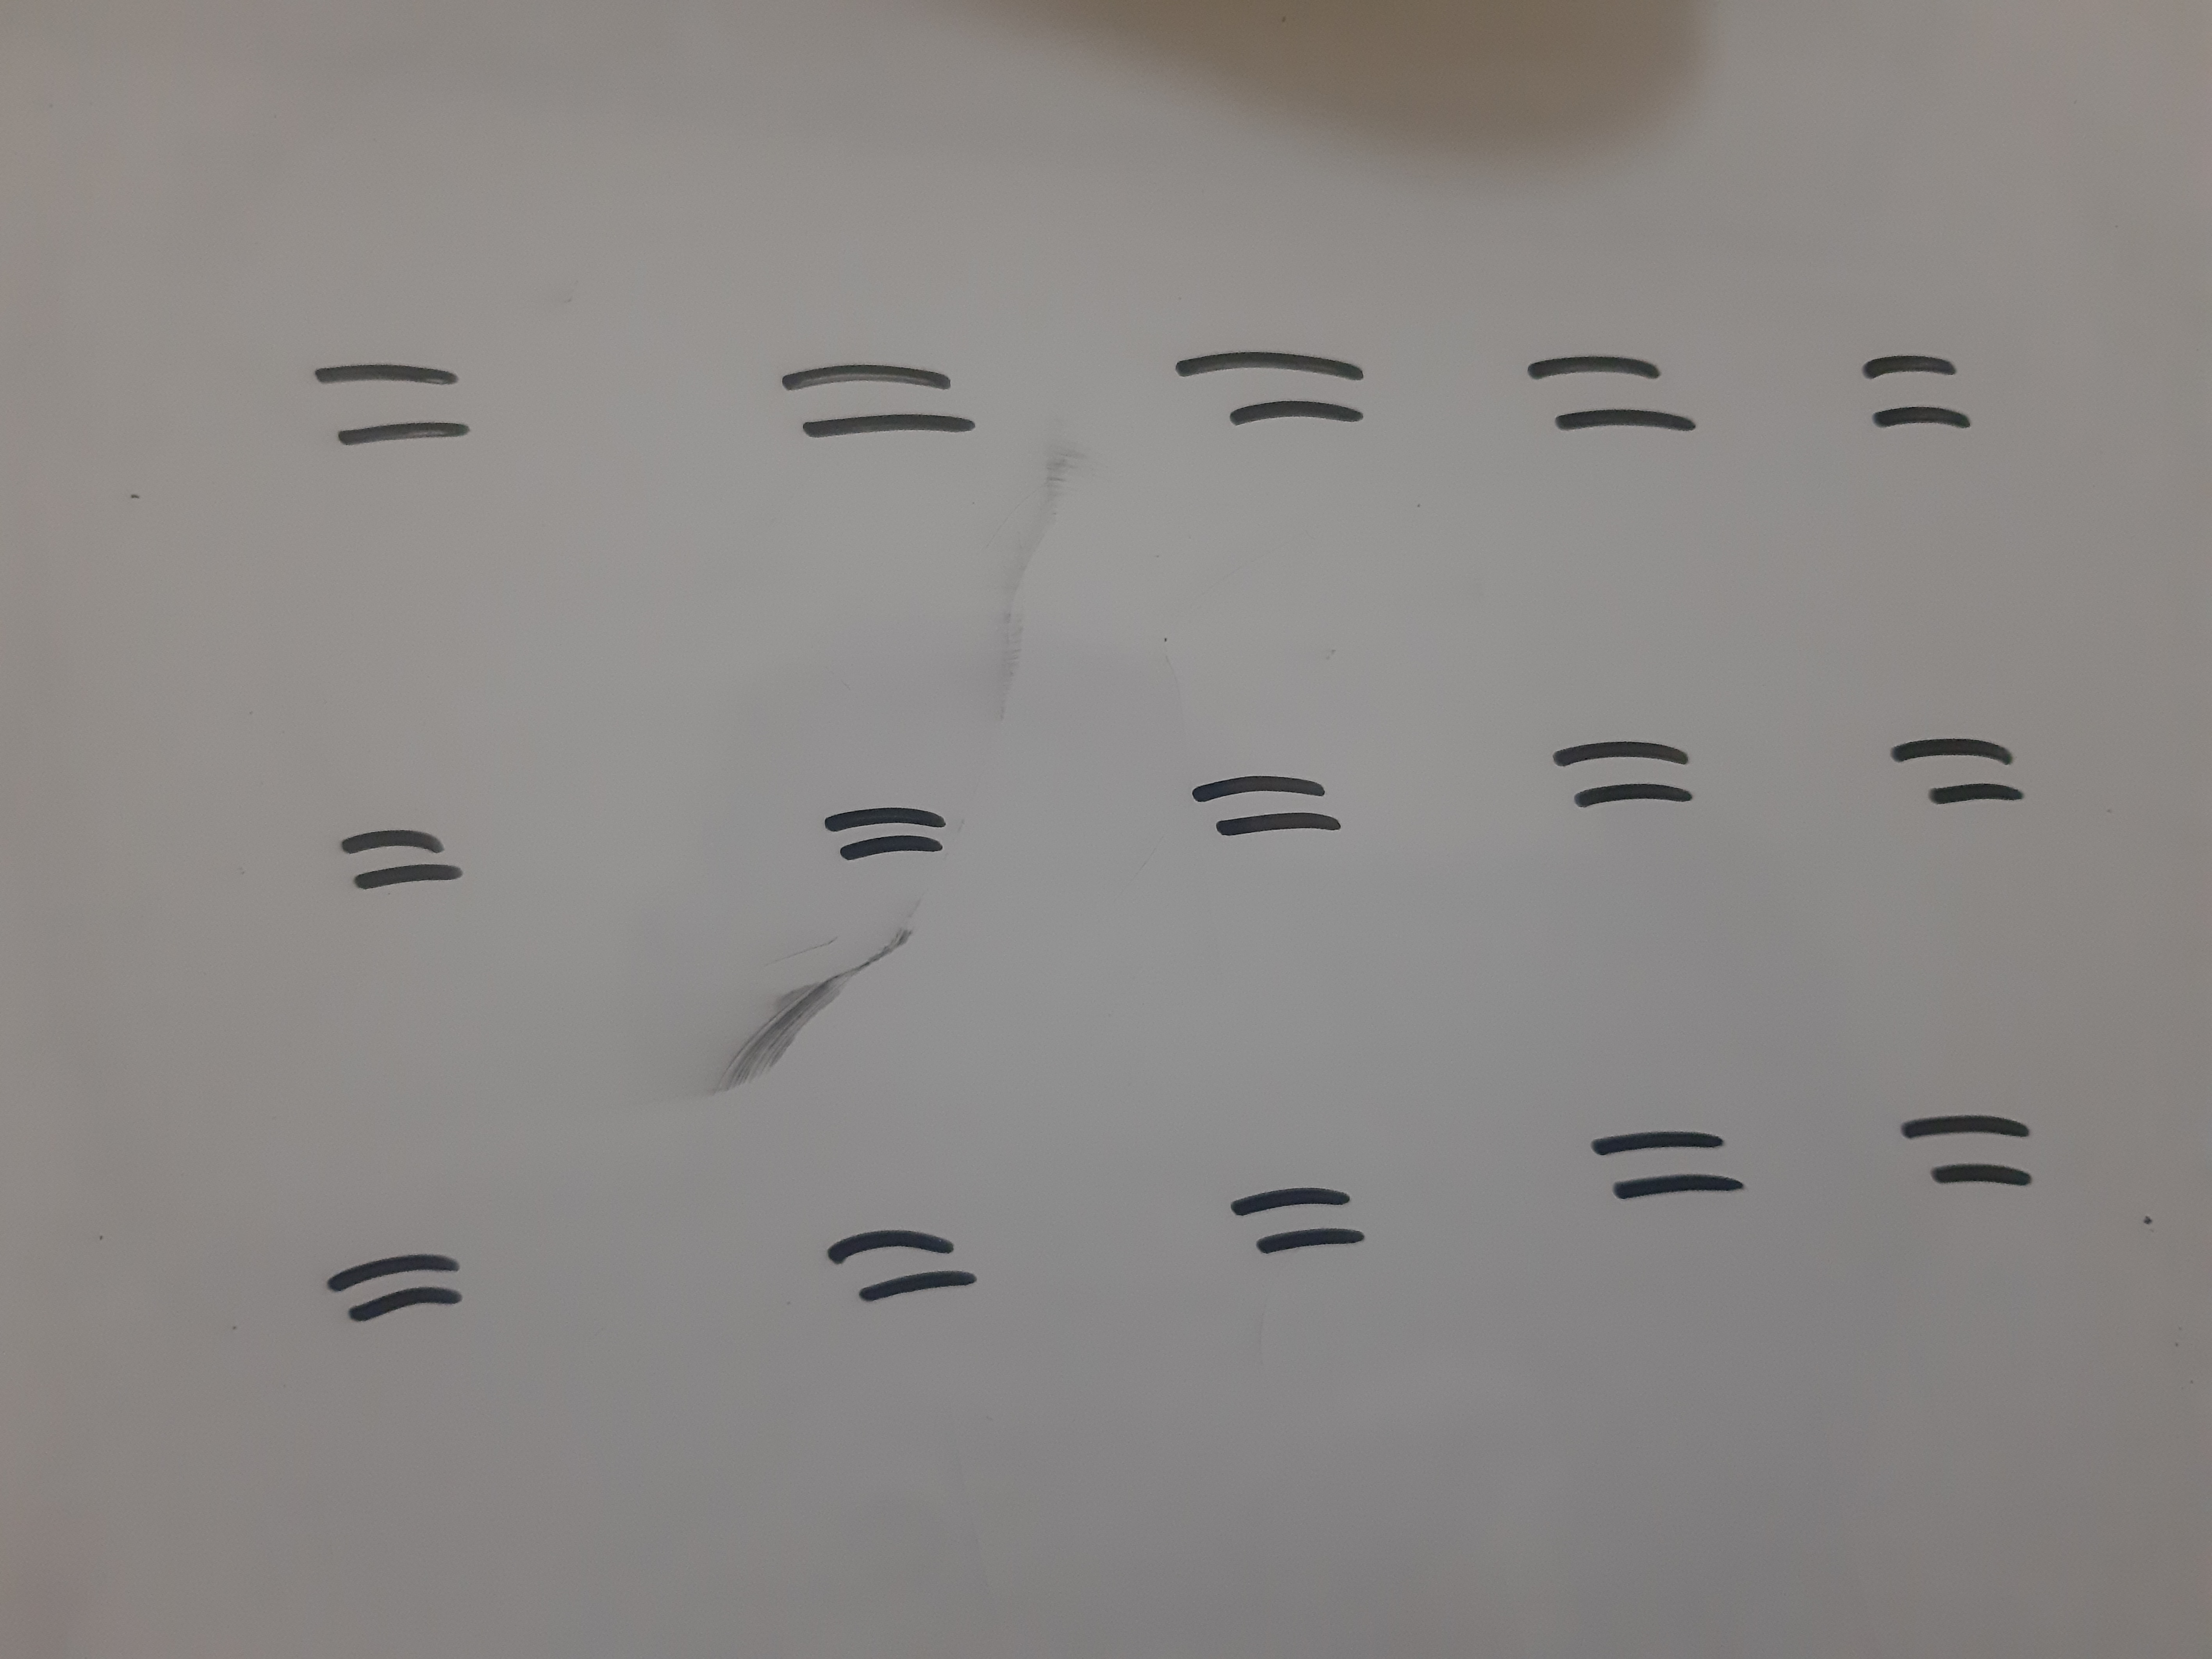
\includegraphics[width=.85\linewidth]{gambar/pengambilan_citra_terang.jpg}
    \caption{Sampel 1, Pengambilan Citra Jarak 30 Cm}
    \label{fig:citra130cm}
  \end{subfigure}%
  \begin{subfigure}{.5\textwidth}
    \centering
    \captionsetup{width=.8\linewidth}
    \includegraphics[width=.85\linewidth]{gambar/pengambilan_citra_gelap.jpg}
    \caption{Sampel 2, Pengambilan Citra Jarak 30 Cm}
    \label{fig:citra230cm}
  \end{subfigure}
  \caption{Pengambilan Citra Jarak 30 Cm}
  \label{fig:citra30cm}
\end{figure}

% 40cm
\begin{figure}[H]
  \begin{subfigure}{.5\textwidth}
    \centering
    \captionsetup{width=.8\linewidth}
    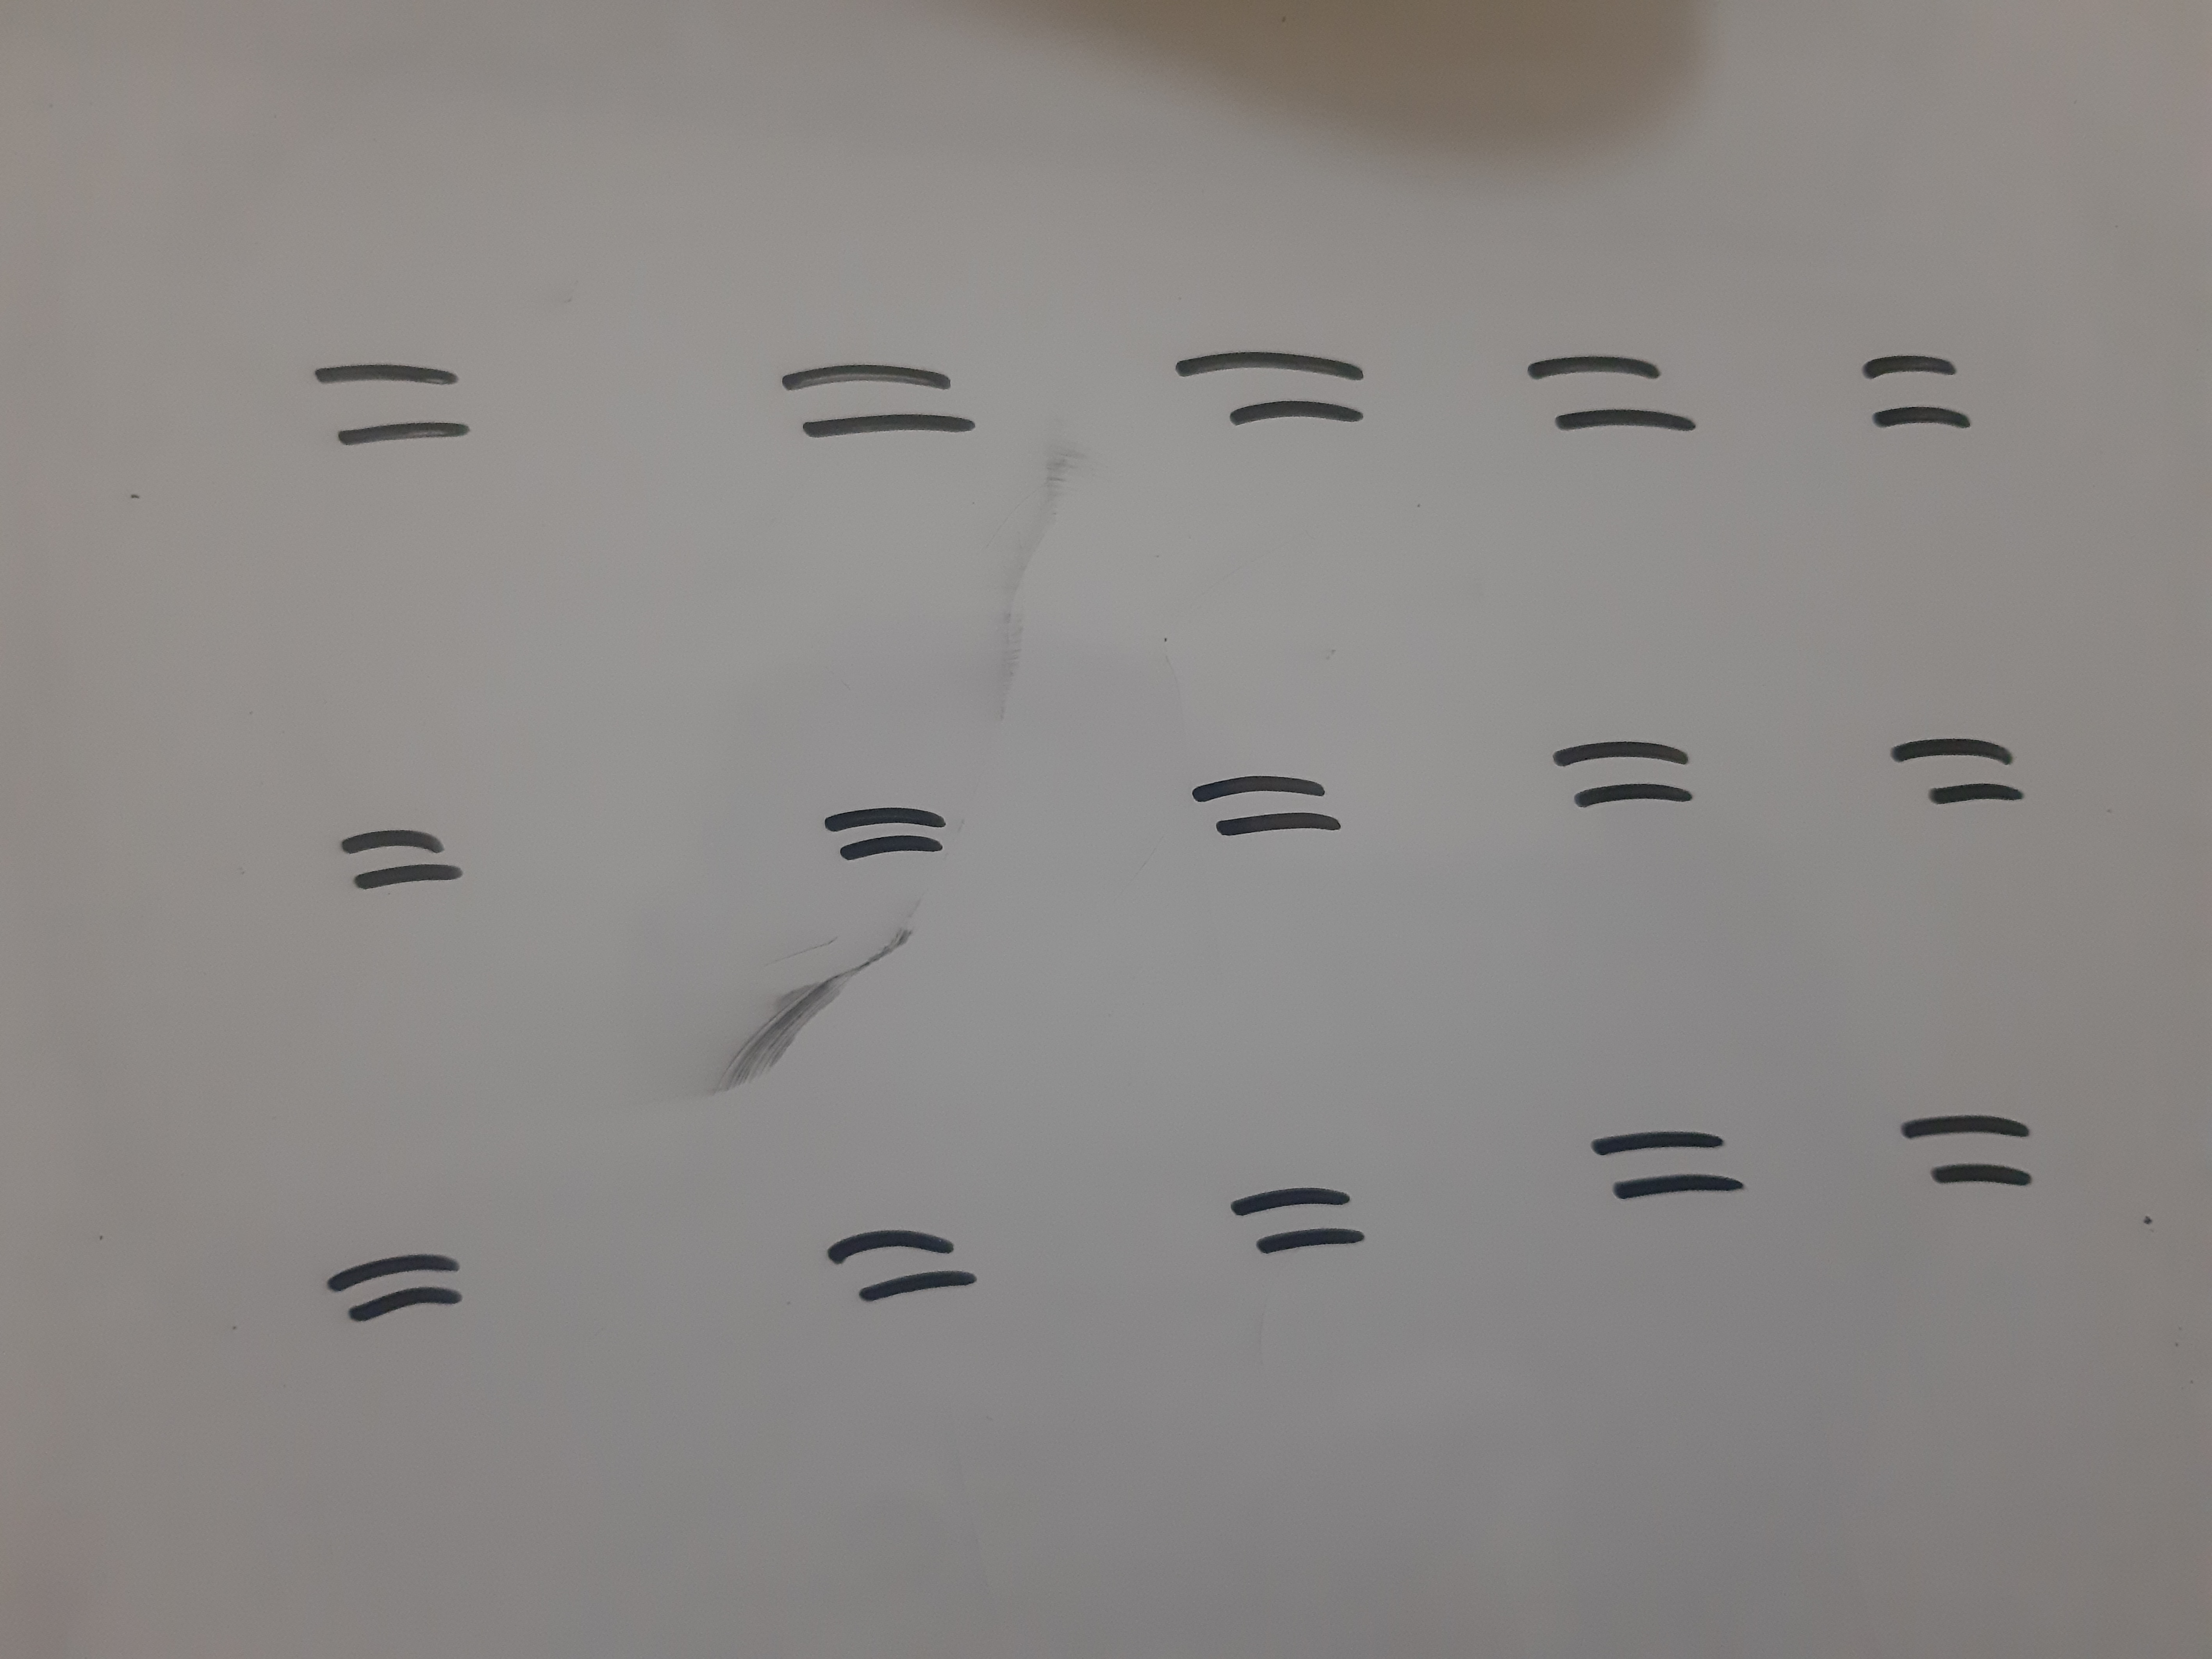
\includegraphics[width=.85\linewidth]{gambar/pengambilan_citra_terang.jpg}
    \caption{Sampel 1, Pengambilan Citra Jarak 40 Cm}
    \label{fig:citra140cm}
  \end{subfigure}%
  \begin{subfigure}{.5\textwidth}
    \centering
    \captionsetup{width=.8\linewidth}
    \includegraphics[width=.85\linewidth]{gambar/pengambilan_citra_gelap.jpg}
    \caption{Sampel 2, Pengambilan Citra Jarak 40 Cm}
    \label{fig:citra240cm}
  \end{subfigure}
  \caption{Pengambilan Citra Jarak 40 Cm}
  \label{fig:citra40cm}
\end{figure}

\subsection{Pengujian Menggunakan \textit{Input} Citra dengan Pencahayaan Pengambilan Citra Bervariasi}
\label{subsec:pengujiancitrabedaintensitas}

Pada pengujian keempat yaitu pengujian dengan menggunakan \textit{input} citra dengan pencahayaan pengambilan citra bervariasi. Tujuan dari pengujian ini yaitu untuk mengetahui pengaruh akurasi model ketika citra yang akan diberikan diambil dengan kondisi pencahayaan yang beragam, serta untuk mengetahui pengaruh pencahayaan dalam pengambilan citra dengan performa dari model. Adapun pada pengujian ini, pengaturan pencahayaan diatur menggunakan fungsi \textit{apperture} yang ada pada kamera. \textit{Apperture} pada kamera untuk pengambilan citra diatur dengan kondisi yaitu kondisi \textit{default} dan juga dengan kondisi \textit{exposure} -1.5 \textit{steps.} Perbandingan hasil pembacaan model terhadap variasi pencahayaan didapatkan hasil yaitu seperti pada Gambar \ref*{fig:citracahayavariasi1}, Gambar \ref*{fig:citracahayavariasi2}, dan Gambar \ref*{fig:citracahayavariasi3} berikut.
% exposure 0 dan -1.5
% //FIXME: ganti gambar, versi terang n gelap dari 2 konten isi sama (sama penulis, sama konten)

% pengujian 1
\begin{figure}[H]
  \begin{subfigure}{.5\textwidth}
    \centering
    \captionsetup{width=.8\linewidth}
    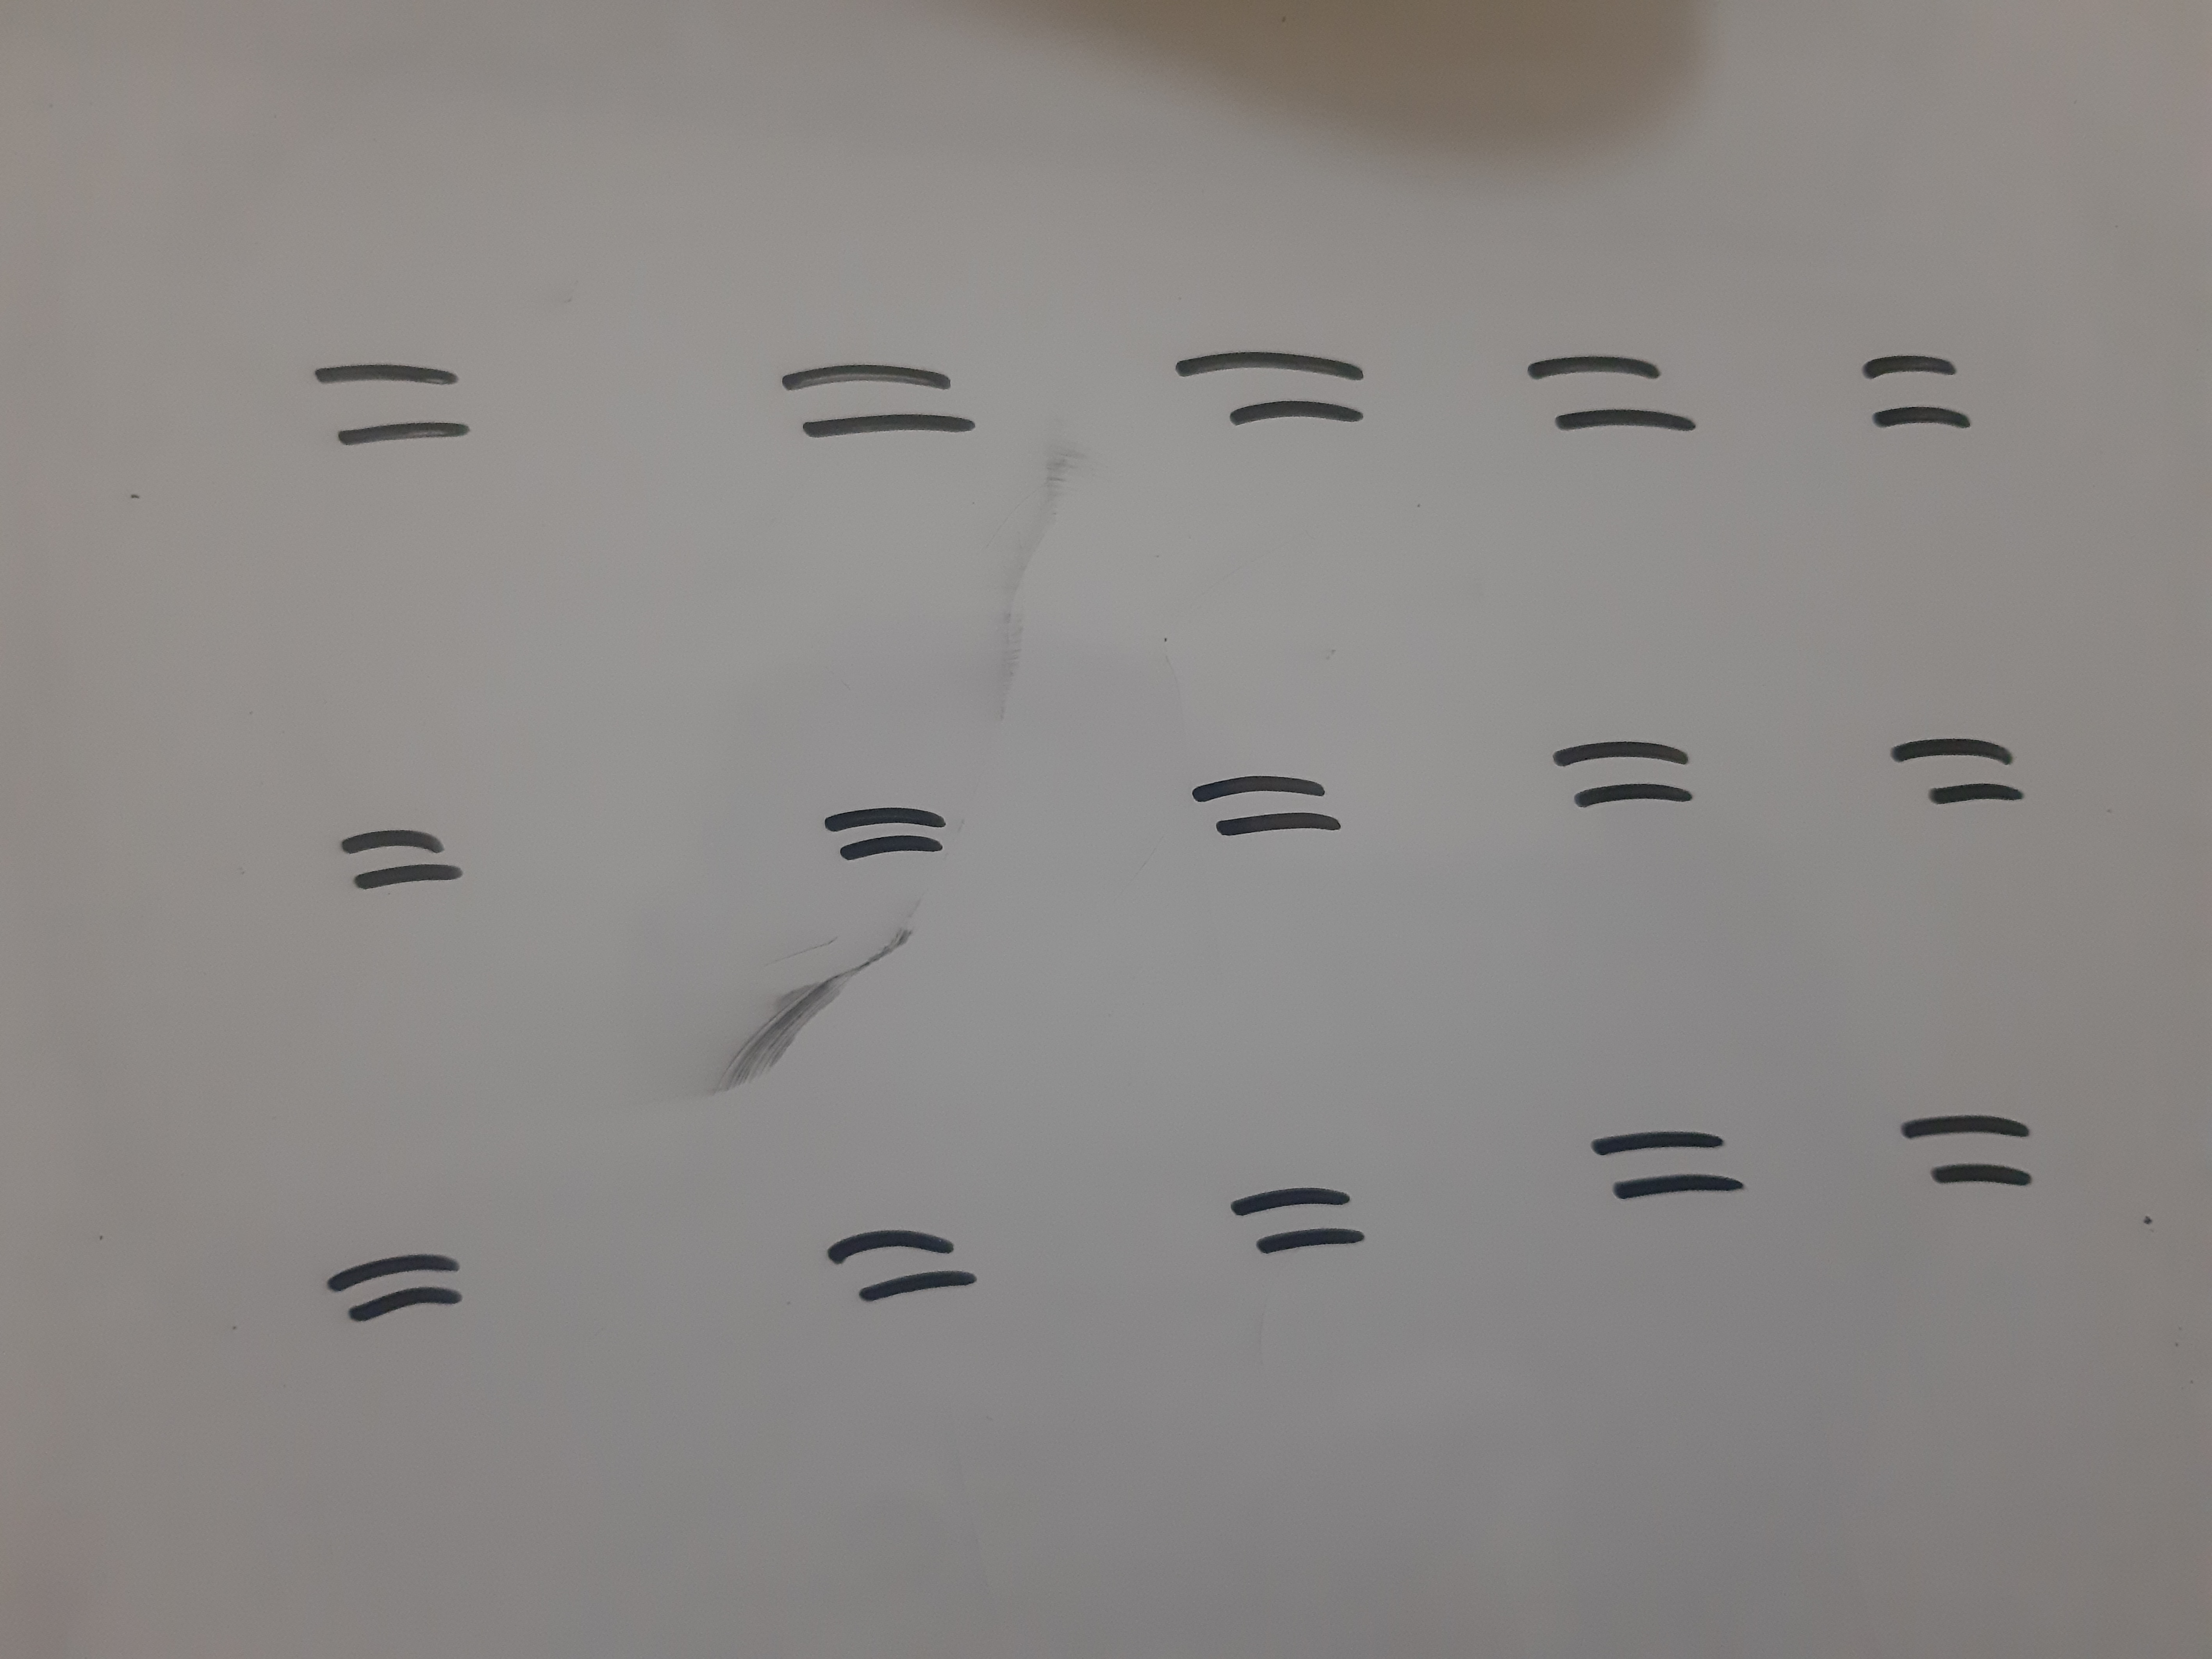
\includegraphics[width=.85\linewidth]{gambar/pengambilan_citra_terang.jpg}
    \caption{Pengambilan Citra Pencahayaan Normal}
    \label{fig:1citracahaya0}
  \end{subfigure}%
  \begin{subfigure}{.5\textwidth}
    \centering
    \captionsetup{width=.8\linewidth}
    \includegraphics[width=.85\linewidth]{gambar/pengambilan_citra_gelap.jpg}
    \caption{Pengambilan Citra Pencahayaan \textit{Apperture} -1 \textit{Steps.}}
    \label{fig:1citracahayamin10}
  \end{subfigure}
  \caption{Pengujian 1, Citra dengan Pencahayaan Berbeda}
  \label{fig:citracahayavariasi1}
\end{figure}

% pengujian 2
\begin{figure}[H]
  \begin{subfigure}{.5\textwidth}
    \centering
    \captionsetup{width=.8\linewidth}
    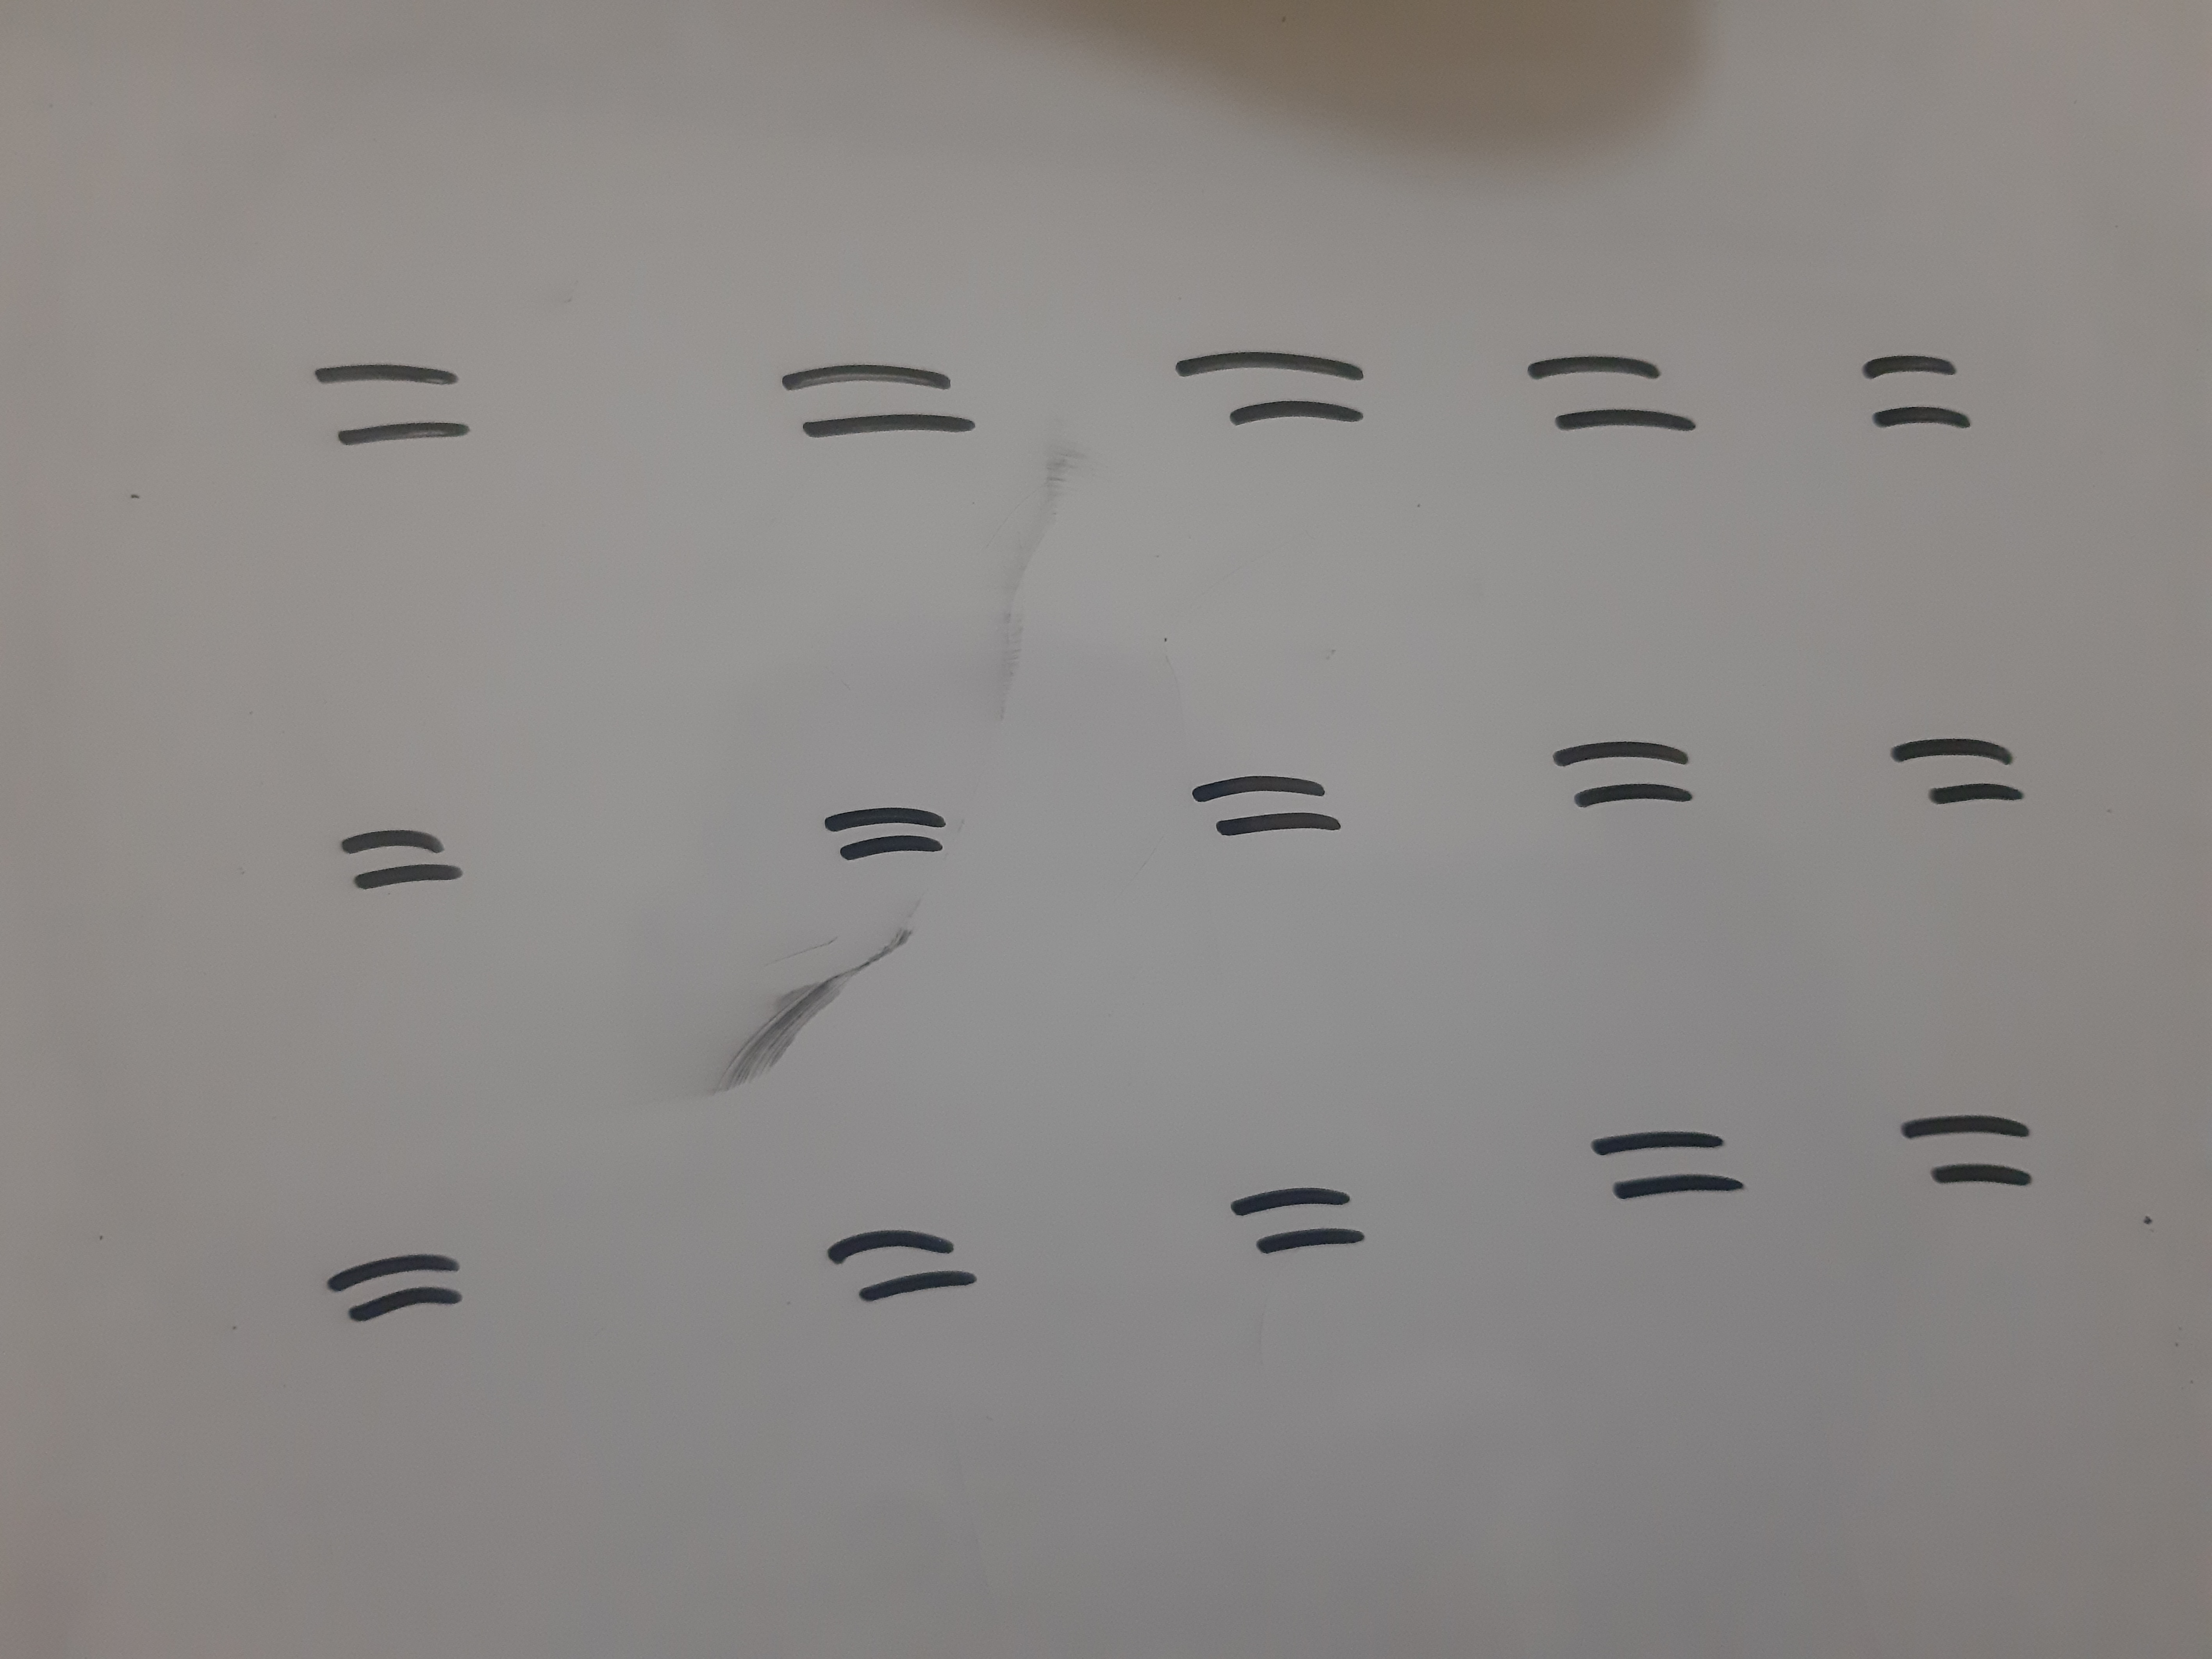
\includegraphics[width=.85\linewidth]{gambar/pengambilan_citra_terang.jpg}
    \caption{Pengambilan Citra Pencahayaan Normal}
    \label{fig:2citracahaya0}
  \end{subfigure}%
  \begin{subfigure}{.5\textwidth}
    \centering
    \captionsetup{width=.8\linewidth}
    \includegraphics[width=.85\linewidth]{gambar/pengambilan_citra_gelap.jpg}
    \caption{Pengambilan Citra Pencahayaan \textit{Apperture} -1 \textit{Steps.}}
    \label{fig:2citracahayamin10}
  \end{subfigure}
  \caption{Pengujian 2, Citra dengan Pencahayaan Berbeda}
  \label{fig:citracahayavariasi2}
\end{figure}

% pengujian 3
\begin{figure}[H]
  \begin{subfigure}{.5\textwidth}
    \centering
    \captionsetup{width=.8\linewidth}
    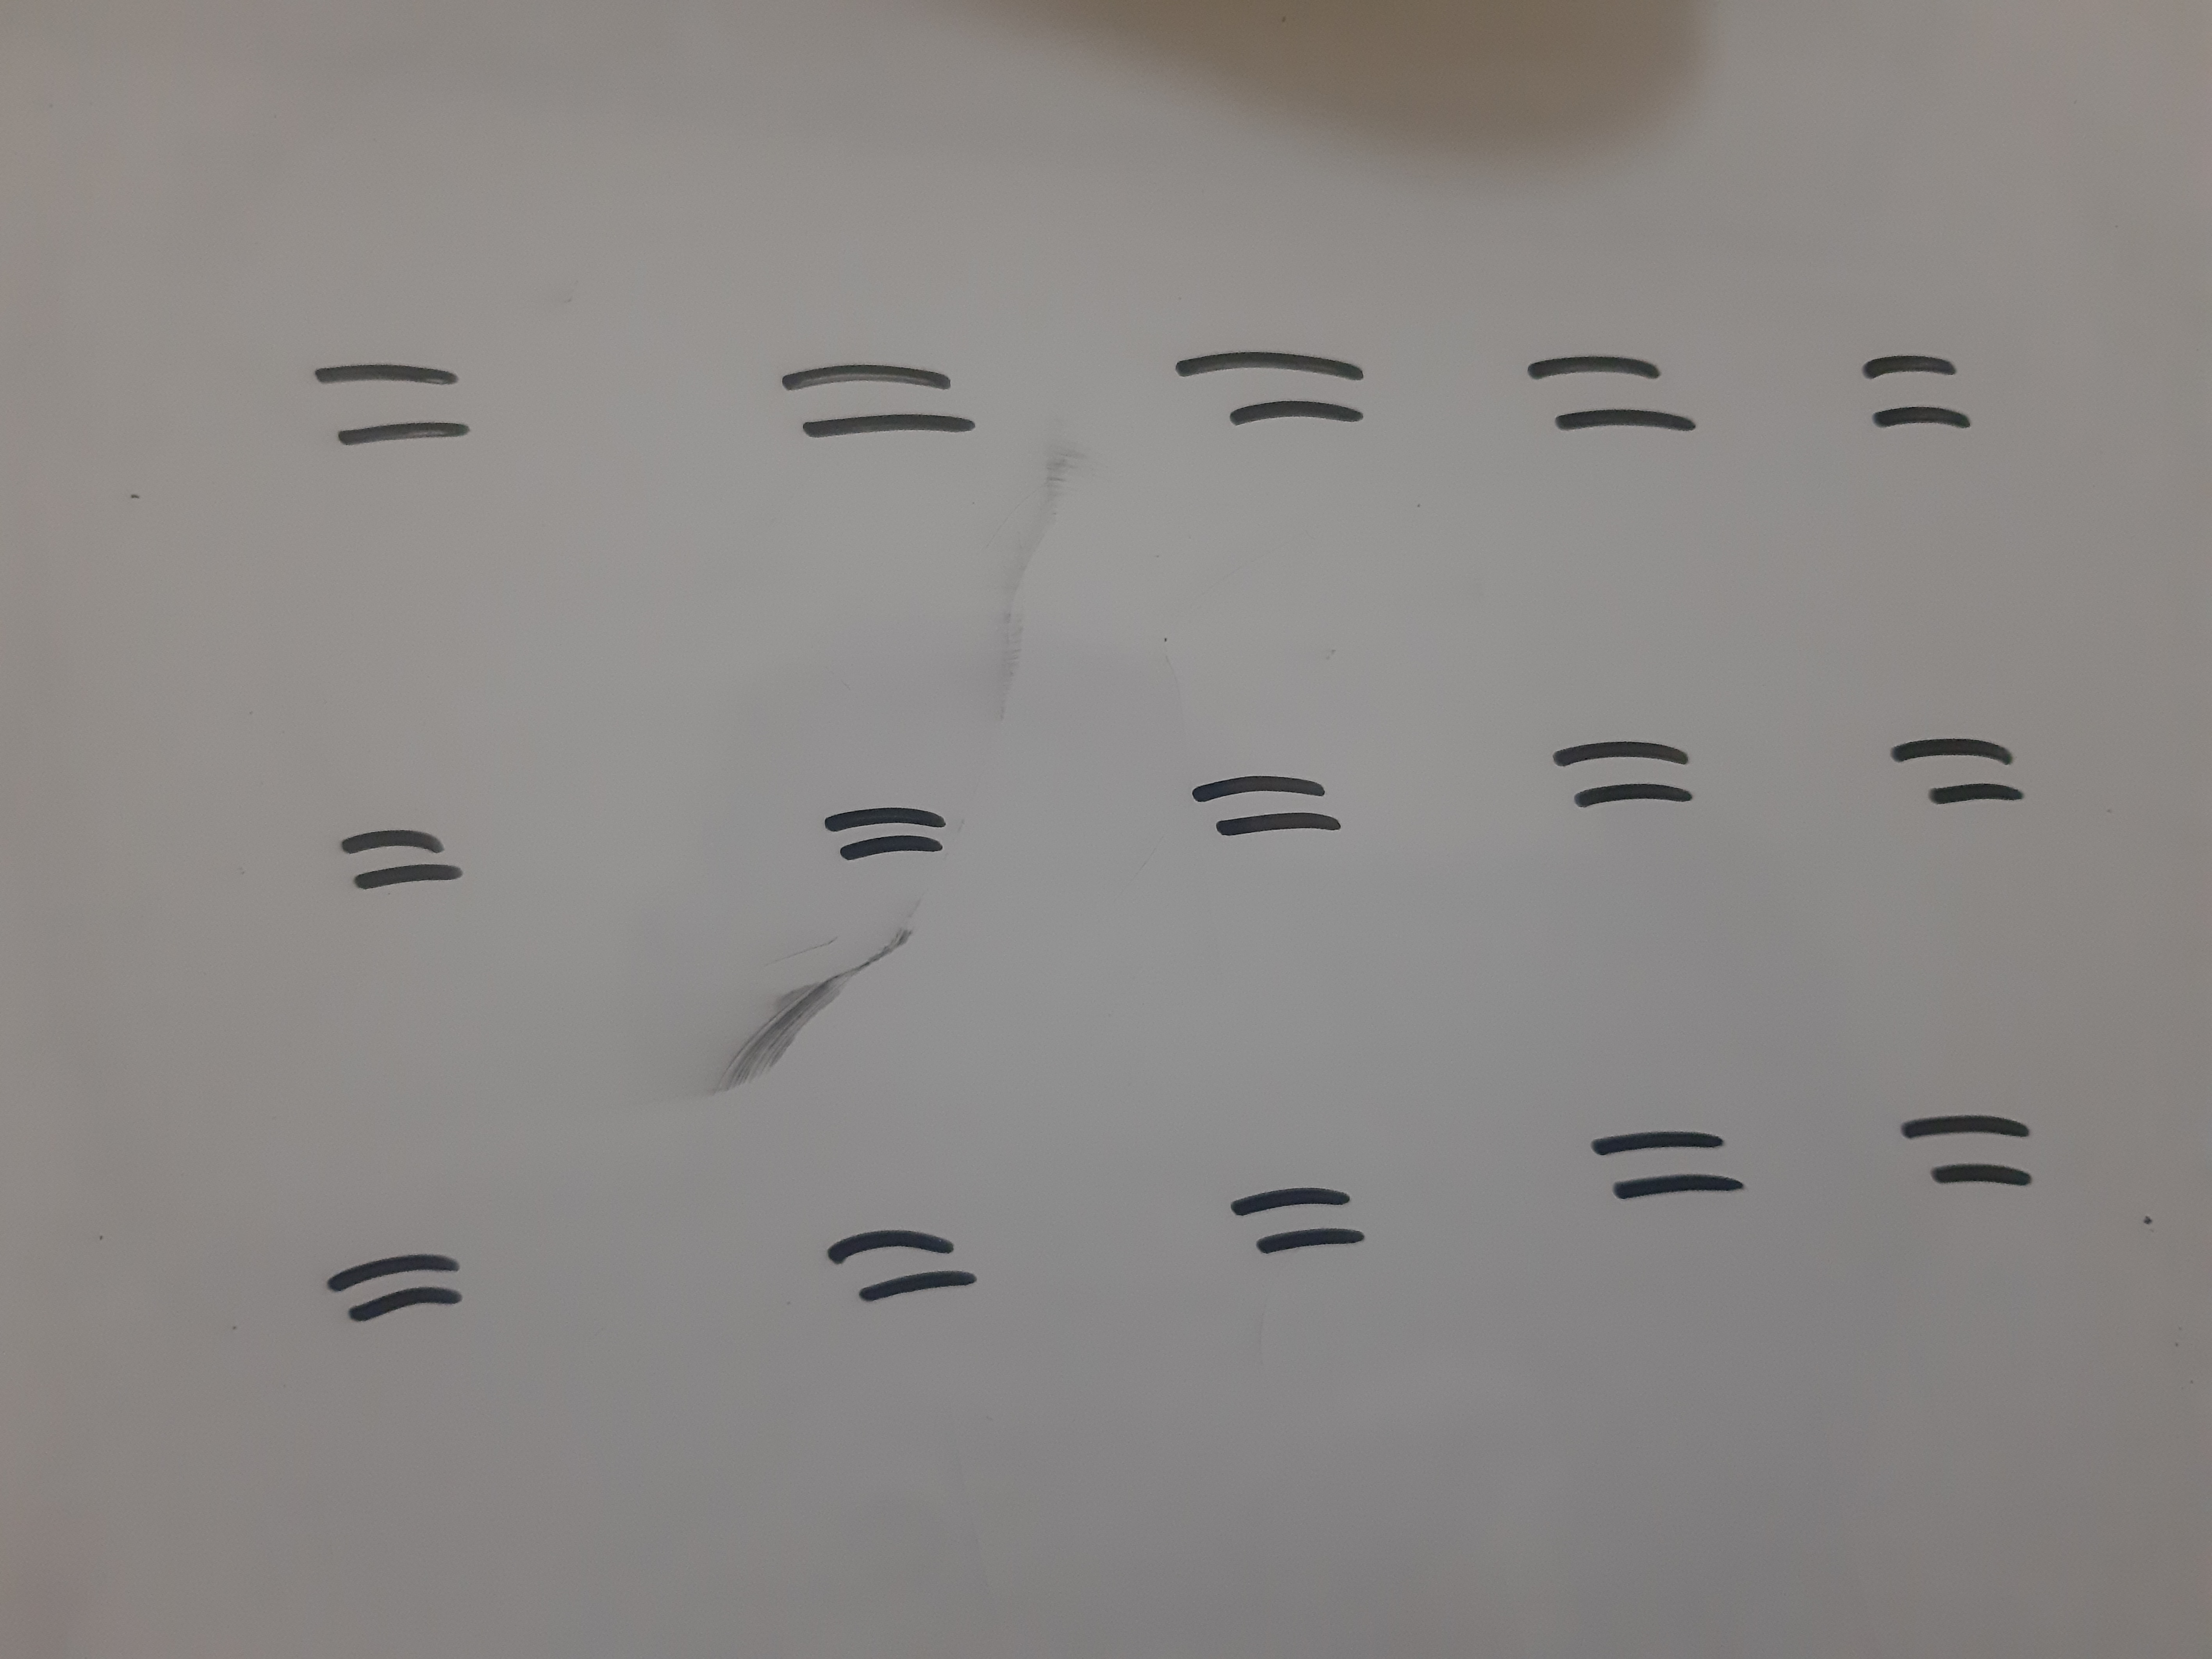
\includegraphics[width=.85\linewidth]{gambar/pengambilan_citra_terang.jpg}
    \caption{Pengambilan Citra Pencahayaan Normal}
    \label{fig:3citracahaya0}
  \end{subfigure}%
  \begin{subfigure}{.5\textwidth}
    \centering
    \captionsetup{width=.8\linewidth}
    \includegraphics[width=.85\linewidth]{gambar/pengambilan_citra_gelap.jpg}
    \caption{Pengambilan Citra Pencahayaan \textit{Apperture} -1 \textit{Steps.}}
    \label{fig:3citracahayamin10}
  \end{subfigure}
  \caption{Pengujian 3, Citra dengan Pencahayaan Berbeda}
  \label{fig:citracahayavariasi3}
\end{figure}

% \section{Evaluasi Pengujian}
% \label{sec:analisispengujian}

% % //FIXME: gatau harus dipakai atau tidak
% \subsection{Evaluasi Pengujian \textit{Training}}
% \label{subsec:evaluasitraining}

% \subsection{Evaluasi Pengujian Menggunakan \textit{Pretrained Weight} Berbeda}
% \label{subsec:evaluasipengujianpretrainedweight}

% \subsection{Evaluasi Pengujian Menggunakan \textit{Input} Citra Tulisan dari Penulis Berbeda}
% \label{subsec:evaluasipengujiancitrabedapenulis}

% \subsection{Evaluasi Pengujian Menggunakan \textit{Input} Citra dengan Jarak Pengambilan Citra Bervariasi}
% \label{subsec:evaluasipengujiancitrabedajarak}

% \subsection{Evaluasi Pengujian Menggunakan \textit{Input} Citra dengan Intensitas Pengambilan Citra Bervariasi}
% \label{subsec:evaluasipengujiancitrabedaintensitas}
